\hypertarget{solutions-des-exercices}{%
\chapter{Etude théorique des solutions}\label{solutions-des-exercices}}

\hypertarget{exercices-essentiels}{%
\section{Exercices essentiels}\label{exercices-essentiels}}

\hypertarget{answer-glob_sol}{%
\subsubsection*{Solutions globales I}\label{answer-glob_sol}}

\addcontentsline{toc}{subsubsection}{Solutions globales I}

Fixons une condition initiale dans \(\mathbb{R}\times \mathbb{R}^2\). La
fonction
\(f:(t,x_1,x_2)\mapsto (\sin x_1 - \sqrt{|t|} x_2 ,\sqrt{1+x_1^2})\) est
continue sur \(\mathbb{R}\times\mathbb{R}^2\). Donc d'après le théorème
de Peano des solutions existent. D'après le théorème du domaine maximal
d'existence, les solutions maximales sont définies sur un intervalle de
temps \(I\) ouvert.

Par ailleurs, on peut vérifier que pour tout \(y\in \mathbb{R}\),
\(\sqrt{1+y^2}\leq 1+|y|\), donc \[
|f_1(x)| \leq 1 + \sqrt{|t|} |x_2| \quad , \quad |f_2(x)|\leq 1 + |x_1|
\] et \(f\) est bornée par une fonction affine en \(\|x\|\). Toutes les
solutions maximales sont donc globales, i.e.~\(I=\mathbb{R}\).

\hypertarget{answer-glob_sol2}{%
\subsubsection*{Solutions globales II}\label{answer-glob_sol2}}

\addcontentsline{toc}{subsubsection}{Solutions globales II}

Considérons une condition initiale dans
\(\mathbb{R}\times \mathbb{R}^n\) et une solution maximale
\(t\mapsto x(t)\) définie sur un intervalle \(I\) (qui existe d'après le
théorème de Peano car \(f\) est continue sur
\(\mathbb{R}\times \mathbb{R}^n\)). Alors \[
\frac{d}{dt} V(x(t)) = \langle\nabla V (x(t)), f(t,x(t))\rangle \leq a(t) V(x(t)) + b(t) \quad \forall t\in I \ ,
\] et donc \[
\frac{d}{dt} \left[e^{-\int_{t_0}^t a(\tau) d\tau}  V(x(t))\right] \leq e^{-\int_{t_0}^t a(\tau) d\tau} b(t)  \quad \forall t\in I \ .
\] En intégrant entre \(t_0\) et \(t\geq t_0\), \[
e^{-\int_{t_0}^t a(\tau) d\tau} V(x(t)) - V(x(t_0)) \leq \int_{t_0}^t e^{-\int_{t_0}^s a(\tau) d\tau} b(s) ds \quad \forall t\in I \cap [t_0,+\infty[
\] et donc \[
V(x(t)) \leq e^{\int_{t_0}^t a(\tau) d\tau} V(x(t_0)) + \int_{t_0}^t e^{\int_{s}^t a(\tau) d\tau} b(s) ds \quad \forall t\in I \cap [t_0,+\infty[ \ .
\] Une autre manière de faire est de montrer que \(V(x(t))\leq v(t)\) où
\(v\) est solution maximale de \[
\dot{v} = a(t) v + b(t)
\] pour la condition initiale \(v(t_0) = V(x(t_0))\), qui est définie
et continue sur \(\mathbb{R}\) car la dynamique de \(v\) est affine.

Or si \(\tmax= \sup I\) est fini, d'après le théorème du domaine
maximal, \((t,x(t))\) tend soit vers la frontière du domaine de
définition de \(f\), soit diverge. Comme \(f\) est définie et continue
sur \(\mathbb{R}\times \mathbb{R}^n\), nécessairement
\(\lim_{t\to \tmax} \|x(t)\| = +\infty\) et donc
\(\lim_{t\to \tmax} V(x(t)) = +\infty\). Or par continuité de \(a,b\)
sur \(\mathbb{R}\), \[
\lim_{t\to \tmax} V(x(t)) \leq e^{\int_{t_0}^{\tmax} a(\tau) d\tau} V(x(t_0)) + \int_{t_0}^{\tmax} e^{\int_{s}^{\tmax} a(\tau) d\tau} b(s) ds   \ .
\] C'est donc impossible et \(\tmax= +\infty\).

\hypertarget{answer-glob_sol3}{%
\subsubsection*{Solutions globales III}\label{answer-glob_sol3}}

\addcontentsline{toc}{subsubsection}{Solutions globales III}

Considérons une condition initiale dans
\(\mathbb{R}\times \mathbb{R}^n\) et une solution maximale
\(t\mapsto x(t)\) définie sur un intervalle \(I\). Alors \[
\frac{d}{dt} V(x(t)) = \langle\nabla V (x(t)), f(t,x(t))\rangle \leq 0 \quad \forall t\in I \ ,
\] donc \(t\mapsto V(x(t))\) décroît et est donc bornée en temps positif
par \(V(x(t_0))\). D'après le théorème du domaine maximal, puisque
\(\mathbb{R}\times \mathbb{R}^n\) n'a pas de frontière, la seule raison
pour laquelle \([t_0,+\infty)\) ne serait pas inclus dans \(I\) serait
que la solution diverge en temps fini. Or c'est impossible car par
hypothèse, on aurait alors \(t\mapsto V(x(t))\) qui diverge. Donc \(x\)
est définie sur \([t_0,+\infty[\). Supposons maintenant qu'elle est non
bornée sur \([t_0,+\infty[\). Alors il existe une suite de temps \((t_n)\)
avec \(\lim_{n\to +\infty} t_n=+\infty\) et
\(\lim_{n\to +\infty} \|x(t_n)\|=+\infty\), et on a
\(\lim_{n\to +\infty} V(x(t_n))=+\infty\), ce qui est impossible. Donc
\(x\) est bien définie et bornée sur \([t_0,+\infty[\).

\hypertarget{answer-ini_sol}{%
\subsubsection*{Unicité de la solution maximale}\label{answer-ini_sol}}

\addcontentsline{toc}{subsubsection}{Unicité de la solution maximale}

Nous avons vu dans l'exercice Solutions globales I que les solutions
maximales de ce système sont définies sur \(\mathbb{R}\). Par ailleurs,
la fonction
\(f:(t,x_1,x_2)\mapsto (\sin x_1 - \sqrt{|t|} x_2 ,\sqrt{1+x_1^2})\) est
continûment différentiable par rapport à \(x\) sur
\(\mathbb{R}\times\mathbb{R}^2\). Donc pour chaque condition initiale
dans \(\mathbb{R}\times\mathbb{R}^2\), il existe une unique solution
maximale.

\hypertarget{answer-crit_stab_dim2}{%
\subsubsection*{Critère de stabilité asymptotique d'un système linéaire
plan}\label{answer-crit_stab_dim2}}

\addcontentsline{toc}{subsubsection}{Critère de stabilité asymptotique d'un système linéaire plan}

Soient \(\lambda_1\) et \(\lambda_2\) les valeurs propres d'une matrice
\(A\) de dimension 2. Son polynôme caractéristique est donné par \[
s^2 - \text{tr} A s + \det A = (s-\lambda_1)(s-\lambda_2) = s^2 - (\lambda_1+\lambda_2)  s + \lambda_1\lambda_2 \ .
\] Donc \(\text{tr} A = \lambda_1+\lambda_2\) et
\(\det A = \lambda_1\lambda_2\). Il y a deux cas: soit les valeurs
propres sont complexes conjuguées, soit elles sont réelles.

Si \(\lambda_i = \lambda_0 \pm j\omega\), alors
\(\lambda_1\lambda_2=\lambda_0^2+\omega^2\) et
\(\lambda_1+\lambda_2 = 2\lambda_0\). Donc \(\lambda_0<0\) si et
seulement si \(\text{tr} A <0\) (et on a alors toujours \(\det A>0\)).

Si les valeurs propres sont réelles, les avoir toutes deux strictement
négatives implique que \(\lambda_1\lambda_2>0\) et
\(\lambda_1+\lambda_2<0\). Réciproquement, si \(\lambda_1\lambda_2>0\),
elles sont non nulles et du même signe, et si de plus
\(\lambda_1+\lambda_2<0\), ce signe est nécessairement négatif.

Donc dans tous les cas, \(\lambda_i\) à parties réelles strictement
négatives équivaut à \(\text{tr} A <0\) et \(\det A>0\).

\hypertarget{answer-ressort-1}{%
\subsubsection*{Oscillateurs couplés I}\label{answer-ressort-1}}

\addcontentsline{toc}{subsubsection}{Oscillateurs couplés I}

Prenons \(x=(y_1,\dot{y}_1,y_2,\dot{y}_2)\) qui vérifie \[
\dot{x} = 
\left(
\begin{matrix}
x_2\\
-\frac{k_1}{m_1} x_1 -\frac{\lambda_1}{m_1} x_2 + \frac{k_{12}}{m_1}(x_3-x_1) \\
x_4\\
-\frac{k_2}{m_2} x_3 -\frac{\lambda_2}{m_2} x_4 - \frac{k_{12}}{m_2}(x_3-x_1) \\
\end{matrix}
\right) 
=
A x
\] avec
\(A=\left( \begin{matrix} 0&1&0&0\\ -\frac{k_1+k_{12}}{m_1}&-\frac{\lambda_1}{m_1}& \frac{k_{12}}{m_1} &0 \\ 0&0&0&1\\ \frac{k_{12}}{m_2}& 0 &-\frac{k_2+k_{12}}{m_2}&-\frac{\lambda_2}{m_2} \end{matrix} \right)\).
Pour avoir un point d'équilibre, il faut \(x_2=x_4=0\) et \[
\left(
\begin{matrix}
-\frac{k_1+k_{12}}{m_1}& \frac{k_{12}}{m_1} \\
\frac{k_{12}}{m_2} &-\frac{k_2+k_{12}}{m_2}
\end{matrix}
\right)
\left(
\begin{matrix}
x_1 \\ x_3
\end{matrix}
\right)
=0
\] dont la seule solution est \(x_1=x_3=0\) (matrice inversible). Donc
le seul point d'équilibre est \(x=(0,0,0,0)\). Vu que l'on a un système
linéaire, les solutions sont uniques, définies sur \(\mathbb{R}\) et
s'écrivent \(x(t) = \exp(At)x(0)\).

Si l'on savait calculer les valeurs propres de \(A\) en fonction des
paramètres, on pourrait en déduire le comportement des solutions et la
stabilité des points d'équilibre.

Lorsque les paramètres des deux masses sont identiques, c'est possible.
En effet, le changement de variable linéaire inversible
\(z=(x_1+x_3,x_2+x_4,x_1-x_3,x_2-x_4)=Px\) donne des dynamiques
découplées de deux oscillateurs indépendants. En effet,
\(\dot{z}=\Sigma z=PAP^{-1}z\) avec
\(\Sigma=\left( \begin{matrix} 0&1&0&0\\ -\frac{k}{m}&-\frac{\lambda}{m}& 0 &0 \\ 0&0&0&1\\ 0& 0 &-\frac{3 k}{m}&-\frac{\lambda}{m} \end{matrix} \right)\)
qui est diagonale par bloc. On peut donc facilement étudier les valeurs
propres de chacun des deux sous-systèmes \(2\times 2\).

Si \(\lambda>0\), on a les traces égales à \(-\frac{\lambda}{m}<0\) et
les déterminants égaux respectivement à \(\frac{k}{m}>0\) et
\(\frac{3k}{m}>0\). Donc d'après l'exercice
\protect\hyperlink{answer-crit_stab_dim2}{Critère de stabilité
asymptotique d'un système linéaire plan (p. \pageref*{answer-crit_stab_dim2})},
chacune des sous-matrices est de Hurwitz, donc \(\Sigma\) l'est aussi,
et donc \(A\) aussi car elles sont semblables. Il s'ensuit que 0 est
globalement asymptotiquement stable. On peut aussi calculer
explicitement les valeurs propres et vérifier qu'elles sont à partie
réelle strictement négative.

Lorsque \(\lambda=0\), les frottements sont absents et les valeurs
propres sont \(\pm i \sqrt{\frac{k}{m}}\) et
\(\pm i \sqrt{\frac{3k}{m}}\). Comme le système est linéaire, on peut
dire que 0 n'est pas attractif donc pas asymptotiquement stable. Mais par
contre, il est bien stable. En effet, vu l'expression des solutions,
elles s'expriment comme des combinaisons linéaires de \(\sin\) et
\(\cos\) aux pulsations \(\sqrt{\frac{k}{m}}\) et
\(\sqrt{\frac{3k}{m}}\). En d'autres termes, le système oscille avec une
superposition de ces fréquences suivant la condition initiale. Il existe
donc \(M\) tel que \[
\|x(t)\|\leq M \|x(0)\| \quad \forall t \in \mathbb{R}\ ,
\] et le point d'équilibre est \emph{stable} au sens de la définition.

NB~: On aurait pu retrouver ce résultat de stabilité en appliquant un
critère de stabilité linéaire sur la matrice \(\Sigma\) (voir
\protect\hyperlink{rem-crit_stabLin}{Remarque (p.
\pageref*{rem-crit_stabLin})}) en disant qu'il y a 4 valeurs propres
(complexes) distinctes donc les sous-espaces propres des valeurs propres
à partie réelle nulle sont tous de dimension 1, égale à leur
multiplicité algébrique.

\hypertarget{answer-asymp_glob-1}{%
\subsubsection*{Stabilité asymptotique I}\label{answer-asymp_glob-1}}

\addcontentsline{toc}{subsubsection}{Stabilité asymptotique I}

La jacobienne de la dynamique est donnée par \[
J_f(x_1,x_2) = 
\left(
\begin{matrix}
0 & 1-3x_2^2 \\
-1+3x_1^2+2x_1x_2 & -(1-x_1^2)
\end{matrix}
\right)
\] soit \[
J_f(0,0) = 
\left(
\begin{matrix}
0 & 1 \\
-1 & -1
\end{matrix}
\right)
\] qui est de Hurwitz (valeurs propres \(\frac{-1\pm i \sqrt{3}}{2}\)).
Donc \((0,0)\) est bien localement asymptotiquement stable. Cependant,
il ne l'est pas globalement car \((1,1)\) est aussi un point
d'équilibre~: la fonction constante égale à \((1,1)\) est solution (et
ne tend pas vers 0).

\hypertarget{answer-ressort-2}{%
\subsubsection*{Oscillateurs couplés II}\label{answer-ressort-2}}

\addcontentsline{toc}{subsubsection}{Oscillateurs couplés II}

L'énergie mécanique du système s'écrit \[
V(x)
= \frac{1}{2} k_1 x_1^2 + \frac{1}{2} k_2 x_3^2 + \frac{1}{2} k_{12} (x_1-x_3)^2 + \frac{1}{2} m_1 x_2^2 + \frac{1}{2} m_2 x_4^2 \ .
\] Il s'agit d'une fonction à valeurs positives, et telle que \(V(x)=0\)
équivaut à \(x=0\). Si on considère une solution \(x\), on calcule \[
\frac{d}{dt} V(x(t)) = -\lambda_1 x_2(t)^2 - \lambda_2 x_4(t)^2 \leq 0 \ .
\] D'après le \protect\hyperlink{stab_decroissance}{théorème de
stabilité par décroissance d'une fonction définie positive (p.
\pageref*{stab_decroissance})}, la position d'équilibre 0 est donc
stable.

Par ailleurs, on voit que \(V\) étant décroissante le long des
solutions, elle est bornée le long des solutions. Vu que
\(\lim_{\|x\|\to \infty} V(x)=+\infty\), on en déduit que les solutions
maximales sont bornées sur \([0,+\infty[\). En effet, s'il existait une
suite de temps \((t_n)\) avec \(\lim_{n\to +\infty} t_n=+\infty\) et
\(\lim_{n\to +\infty} \|x(t_n)\|=+\infty\), on aurait
\(\lim_{n\to +\infty} V(x(t_n))=+\infty\), ce qui est impossible.

De plus, vu que \(\dot x = Ax\), les dérivées successives des solutions
s'écrivent comme des combinaisons linéaires des solutions et sont donc
elles aussi toutes bornées sur \([0,+\infty[\).

Soit \(v:[0,+\infty[\to \mathbb{R}\) définie par \(v(t) = V(x(t))\) pour
une solution \(x:[0,+\infty)\to \mathbb{R}^4\). \(v\) est minorée par 0 et
décroissante car \[
\dot{v}(t) = -\lambda_1 x_2(t)^2 - \lambda_2 x_4(t)^2 \leq 0
\] donc elle converge lorsque \(t\) tend vers l'infini. Par ailleurs, \[
\ddot{v}(t) = -2\lambda_1 x_2(t)\dot{x}_2(t) - 2\lambda_2 x_4(t)\dot{x}_4(t) 
\] est bornée vu qu'on a montré que les dérivées successives des
solutions sont bornées. En appliquant le lemme de Barbalat, on en déduit
que \(\dot{v}\) tend vers 0 lorsque \(t\) tend vers l'infini.

Supposons que \(\lambda_1\) est strictement positif. Alors
\(0\leq x_2(t)^2\leq -\frac{\dot{v}(t)}{\lambda_1}\) et la vitesse
\(x_2\) de la première masse tend vers 0. Mais vu que \(\ddot{x}_2\) est
bornée, on a de nouveau par Barbalat que \(\dot x_2\) tend vers zéro,
soit \(- k_1 x_1 - k_{12} (x_1 - x_3)\) tend vers 0. En redérivant et en
réappliquant Barbalat, on obtient alors que
\(- k_1 x_2 - k_{12} (x_2 - x_4)\) tend vers zéro, et vu que \(x_2\)
tend vers 0, \(x_4\) tend vers 0. En redérivant et en réappliquant
Barbalat sur \(x_4\), on obtient que \(- k_2 x_3 + k_{12} (x_1 - x_3)\)
tend vers 0, et donc enfin, en combinant avec
\(- k_1 x_1 - k_{12} (x_1 - x_3)\), les positions \((x_1,x_3)\) tendent
vers 0. On conclut donc finalement que \(\lim_{t\to \infty}x(t) = 0\)
et 0 est globalement attractif. Vu que par ailleurs, il est stable, on
démontre ainsi qu'il est asymptotiquement stable.

On obtient de manière similaire le résultat si \(\lambda_2\) est
strictement positif.

\hypertarget{answer-asymp_glob-2}{%
\subsubsection*{Stabilité asymptotique II}\label{answer-asymp_glob-2}}

\addcontentsline{toc}{subsubsection}{Stabilité asymptotique II}

La jacobienne de la dynamique est donnée par \[
J_f(0,0) = 
\left(
\begin{matrix}
0 & 1 \\
0 & -1
\end{matrix}
\right)
\] qui admet 0 et -1 comme valeurs propres. Nous ne pouvons donc rien
conclure sur la stabilité de 0 par le linéarisé.

Considérons \(V:\mathbb{R}^2\to \mathbb{R}_{\geq 0}\) définie par \[
V(x_1,x_2)= x_1^4 + 2 x_2^2
\] qui est positive et ne s'annule qu'en \(x=0\). De plus, elle vérifie
le long des solutions \[
\frac{d}{dt} V(x(t)) = - 4x_2(t)^2 \leq 0
\] donc \(V\) décroît le long des solutions et 0 est stable.

La décroissance de \(t\mapsto V(x(t))\) implique aussi que
\(t\mapsto V(x(t))\) est bornée, ce qui empêche les solutions de
diverger, car \(\lim_{\|x\|\to +\infty} V(x) = +\infty\). Donc les
solutions ne peuvent pas diverger en temps fini positif, et les
solutions maximales sont définies sur \([0,\infty[\). Elles sont même
bornées (en temps positif), car sinon il existerait une suite de temps
\((t_n)\) avec \(\lim_{n\to +\infty} t_n=+\infty\) et
\(\lim_{n\to +\infty} \|x(t_n)\|=+\infty\), et on aurait
\(\lim_{n\to +\infty} V(x(t_n))=+\infty\), ce qui est impossible. Le
long de n'importe quelle solution maximale \(t\mapsto x(t)\), on a donc
(i) \(v(t)=V(x(t))\) qui décroît et est minoré, donc converge lorsque
\(t\) tend vers l'infini, (ii) \(\dot{v}(t) = - 4x_2^2(t)\), et (iii)
\(\ddot{v}(t)= - 8x_2(t)\dot{x}_2(t)=- 8x_2(t)(-x_1(t)^3-x_2(t))\)
bornée. Donc, par le lemme de Barbalat, \(t\mapsto x_2(t)\) converge
vers 0 lorsque \(t\) tend vers l'infini. Par ailleurs, de manière
similaire, \(\ddot{x}_2(t) = -3x_1^2x_2-(-x_1(t)^3-x_2(t))\) est bornée,
et donc en appliquant Barbalat de nouveau à \(x_2\), on en déduit que
\(\dot{x}_2\) tend vers 0 et donc \(x_1\) tend vers 0. Ainsi, \((0,0)\)
est globalement attractif, et on a vu qu'il est stable, donc il est bien
globalement asymptotiquement stable.

Notons qu'avec l'habitude, on aurait pu considérer la fonction
\(V:\mathbb{R}^2\to \mathbb{R}_{\geq 0}\) définie par \[
V(x_1,x_2)= x_1^4 + x_2^2 + (x_1+x_2)^2
\] qui est aussi positive et ne s'annule qu'en \(x=0\). En effet,
celle-ci a le bon goût de vérifier \begin{align*}
\frac{d}{dt} V(x(t))  
&= 4x_1^3x_2 - 2 x_1^3x_2 - 2x_2^2 + 2(x_1+x_2)(x_2-x_1^3-x_2)\\
&= -2x_2(t)^2 -2 x_1(t)^4 
\end{align*} qui est strictement négatif tant que la solution n'est pas
au point d'équilibre. L'application du Lemme de Barbalat donne alors
directement la convergence de la solution vers 0 sans avoir à
l'appliquer plusieurs fois. En fait dans ce cas, le troisième
\protect\hyperlink{exo_lyap}{\emph{critère de Lyapunov} (p.
\pageref*{exo_lyap})} (\(\langle \nabla V(x) , f(x) \rangle<0\) pour
tout \(x\neq 0\) et \(\lim_{\|x\|\to +\infty} V(x) = +\infty\)) permet
de déduire directement la stabilité asymptotique globale.

\hypertarget{correc_Torricelli}{%
\section{Ecoulement dans un réservoir}\label{correc_Torricelli}}

\hypertarget{answer-tor-1}{%
\subsubsection*{Question 1}\label{answer-tor-1}}

\addcontentsline{toc}{subsubsection}{Question 1}

\(f:(t,x)\mapsto -k\sqrt{|x|}\) est continue sur
\(\mathbb{R}\times \mathbb{R}\) donc le théorème de Peano nous garantit
l'existence de solutions au problème de Cauchy dans \(\mathbb{R}\) pour
toute condition initiale.

De plus, \(\sqrt{|x|}\leq 1+|x|\) pour tout \(x\in \mathbb{R}\) donc
\(f\) est bornée de manière affine et toute solution maximale (dans
\(\mathbb{R}\)) est définie sur \(\mathbb{R}\).

Enfin, \(f\) est continûment différentiable sur
\(\mathbb{R}\times (\mathbb{R}\setminus \{0\})\) donc lorsque
\(x_0\neq 0\), il existe une unique solution maximale dans
\(\mathbb{R}\setminus \{0\}\) d'après le théorème de Cauchy-Lipschitz
(appliqué ici sur l'ouvert \(X=\mathbb{R}\setminus \{0\}\)). Autrement
dit, la solution est unique tant qu'elle reste dans
\(\mathbb{R}\setminus \{0\}\). Par contre, \(f\) n'est pas
différentiable en 0 (ni même lipschitzienne) donc le théorème de
Cauchy-Lipschitz ne s'applique pas sur \(X=\mathbb{R}\)~: on ne peut
plus garantir l'unicité à partir du moment où la solution maximale passe
par 0.

\hypertarget{answer-tor-2}{%
\subsubsection*{Question 2}\label{answer-tor-2}}

\addcontentsline{toc}{subsubsection}{Question 2}

Soit d'abord \(x_0>0\). Tant que \(x(t)>0\), on a \[
\dot{x}=-k\sqrt{|x|} \quad \Leftrightarrow \quad \frac{\dot{x}}{\sqrt{x}}=-k  \quad \Leftrightarrow \quad x(t) = \left(\sqrt{x_0}-\frac{k}{2}(t-t_0)\right)^2
\] Donc tant que \(x(t)>0\), la solution est unique (comme prévu dans la
question précédente) et par continuité, elle atteint 0 en
\(t_1=t_0+2\sqrt{x_0}/k\). A partir de là, une solution est de rester
constamment égale à 0. Sinon, considérons \(t_2\) l'infimum des temps
supérieurs à \(t_1\) tels que \(x(t)\) est non nul. Alors vu que
\(\dot{x}\leq 0\), on a \(x(t)< 0\) pour tout \(t\in ]t_2,+\infty[\).
Sur cet intervalle, \[
\dot{x}=-k\sqrt{|x|} \quad \Leftrightarrow \quad \frac{\dot{x}}{\sqrt{-x}}=-k  \quad \Leftrightarrow \quad x(t) = -\left(\frac{k}{2}(t-t_2)\right)^2
\] On voit alors que toutes les fonctions de ce type avec
\(t_2\geq t_1\) arbitraire sont solutions. Pour \(x_0>0\), l'ensemble
des solutions est donc l'ensemble des fonctions définies par \[
x(t)= 
\left\{
\begin{array}{ll}
\left(\sqrt{x_0}-\frac{k}{2}(t-t_0)\right)^2 & \forall t\in ]-\infty,t_0+2\sqrt{x_0}/k] \\
0 & \forall t\in [t_0+2\sqrt{x_0}/k,t_2] \\
-\left(\frac{k}{2}(t-t_2)\right)^2 & \forall t\in [t_2,+\infty)
\end{array}
\right.
\] pour n'importe quel \(t_2\in [t_0+2\sqrt{x_0}/k,+\infty]\). Il y a
donc une infinité de solutions (unicité du passé et non unicité du
futur).

Maintenant si \(x_0=0\). Pour \(t\geq t_0\), on reproduit le même
raisonnement. De même, pour \(t\leq t_0\), soit \(x\) reste à 0 soit il
existe \(t_1 < t_0\) tel que \(x(t_1)>0\), et on obtient que les
solutions maximales s'écrivent \[
x(t)= 
\left\{
\begin{array}{ll}
\frac{k^2}{4}(t-t_1)^2 & \forall t\in ]-\infty,t_1] \\
0 & \forall t\in [t_1,t_2]\\
-\frac{k^2}{4}(t-t_2)^2 & \forall t\in [t_2,+\infty]
\end{array}
\right.
\] pour n'importe quels \(t_1 \in [-\infty,t_0]\) et
\(t_2 \in [t_0,+\infty]\). Il y a donc une infinité de solutions (à la
fois dans le passé et le futur).

\hypertarget{answer-tor-3}{%
\subsubsection*{Question 3}\label{answer-tor-3}}

\addcontentsline{toc}{subsubsection}{Question 3}

Lorsque \(x_0>0\), il y a une seule solution physique, celle qui va à
zéro et y reste à jamais. Par contre, lorsque \(x_0=0\), il y a une
infinité de passés possibles car lorsqu'on voit le réservoir vide à
\(t_0\) on ne sait pas depuis quand il est vide\ldots{}

\hypertarget{answer-tor-4}{%
\subsubsection*{Question 4}\label{answer-tor-4}}

\addcontentsline{toc}{subsubsection}{Question 4}

Lorsque \(x_0>0\), les solutions sont continues par rapport à la
condition initiale tant qu'elles restent strictement positives (théorème
appliqué sur le domaine \(X= \mathbb{R}\setminus \{0\}\) où \(f\) est
\(C^1\)). Par contre, si \(x_0=0\), une solution possible est
\(x\equiv 0\) alors que pour tout \(\delta>0\), la solution partant de
\(x_0+\delta\) est donnée par
\(x_\delta(t)=\left(\sqrt{x_0+\delta}-\frac{k}{2}(t-t_0)\right)^2\) pour
\(t\leq t_0\). Donc sur un horizon de temps fixé (rétrograde)
\([\underline{t},t_0]\), la différence \(\|x-x_\delta\|\) ne peut être
rendue arbitrairement petite en faisant tendre \(\delta\) vers 0. Le
même phénomène apparaît en temps positif lorsque l'on considère les
solutions négatives. En ce sens, on n'a pas la continuité des solutions
par rapport à la condition initiale. Cela ne contredit pas le théorème
car \(f(x)=-\sqrt{|x|}\) n'est pas \(C^1\), ni lipschitzienne en 0.

\hypertarget{correc_gronwall}{%
\section{Autour du Lemme de Grönwall}\label{correc_gronwall}}

\hypertarget{answer-gro-1}{%
\subsubsection*{Question 1 (Lemme de Grönwall)}\label{answer-gro-1}}

\addcontentsline{toc}{subsubsection}{Question 1 (Lemme de Grönwall)}

Soit \(v\) l'application définie par \(v(t)=\int_{t_0}^t\beta(s)u(s)ds\)
sur \(I\). Elle vérifie \[
\dot{v}(t) = \beta(t)u(t) \quad , \quad u(t) \leq \alpha(t)+v(t) \ ,
\] et donc puisque \(\beta\) est à valeurs positives, \[
\dot{v}(t) \leq \alpha(t)\beta(t)+\beta(t)v(t) \ .
\] Soit maintenant \(w\) l'application définie par
\(w(t)=v(t)\exp\left(-\int_{t_0}^t\beta(r)dr\right)\). \(w\) est
dérivable sur \(I\) et pour tout \(t\in I\), \begin{align*}
\dot{w}(t) &= (\dot{v}(t)-\beta(t)v(t))\exp\left(-\int_{t_0}^t\beta(r)dr\right)\\
&\leq \alpha(t)\beta(t)\exp\left(-\int_{t_0}^t\beta(r)dr\right)
\end{align*} En intégrant des deux côtés entre \(t_0\) et \(t\geq t_0\),
on obtient \[
w(t)-w(t_0)\leq \int_{t_0}^t \alpha(s)\beta(s)\exp\left(-\int_{t_0}^s\beta(r)dr\right)ds
\] et en remplaçant \(w\) par son expression, \[
v(t)\leq \int_{t_0}^t \alpha(s)\beta(s)\exp\left(\int_{s}^t\beta(r)dr\right)ds \ ,
\] ce qui donne le résultat. Finalement, si \(\alpha\) est constant
alors \begin{align*}
u(t) &\leq \alpha +\alpha \left[-\exp\left(\int_s^t\beta(r)dr \right) \right]_{t_0}^t \\
& \leq \alpha -\alpha +\alpha \exp\left(\int_{t_0}^t\beta(r)dr \right)
\end{align*} ce qui donne le résultat.

\hypertarget{answer-gro-2}{%
\subsubsection*{Question 2}\label{answer-gro-2}}

\addcontentsline{toc}{subsubsection}{Question 2}

Soit \(x:I\subset J\to \mathbb{R}^n\) une solution maximale au problème
de Cauchy. Par le théorème de
\protect\hyperlink{theo_eq_integrale}{représentation intégrale des
solutions (p. \pageref*{theo_eq_integrale})}, pour tout \(t\in I\), \[
x(t)=x_0 + \int_{t_0}^t f(s,x(s))ds \ ,
\] et donc, utilisant l'hypothèse de borne au plus affine de \(f\), \[
\|x(t)\| \leq \|x_0\| + \int_{t_0}^t |b(s)| + |a(s)|\|x(s)\|ds 
\] pour tout \(t\in I\) avec \(t\geq t_0\). Le Lemme de Grönwall donne
alors \[
\|x(t)\| \leq \alpha(t) +  \int_{t_0}^{t} \alpha(s)\beta(s) \exp\left(\int_{s}^t\beta(r)dr \right) ds
\] avec \(\alpha(t)=\|x_0\| + \int_{t_0}^t |b(s)| ds\) et
\(\beta(t)= |a(t)|\) qui sont continues sur \(J\). Donc \(x\) ne peut
pas exploser en temps fini supérieurs à \(t_0\) dans \(J\) (le membre de
droite restant borné). En reprenant le raisonnement en temps inférieurs
à \(t_0\) en renversant le temps et considérant \(-f\) au lieu de \(f\),
on obtient que \(x\) ne peut pas non plus exploser en temps fini
inférieurs à \(t_0\) dans \(J\). Donc nécessairement \(I=J\) d'après le
\protect\hyperlink{theo_bouts}{théoreme du domaine maximal d'existence
(p. \pageref*{theo_bouts})}, vu que \(f\) est définie sur
\(J\times\mathbb{R}^n\).

\hypertarget{answer-gro-3}{%
\subsubsection*{Question 3}\label{answer-gro-3}}

\addcontentsline{toc}{subsubsection}{Question 3}

Soient \((t_0,x_0)\in J\times X\) et \(\delta\in \mathbb{R}^n\) tel que
\((t_0,x_0+\delta)\in J\times X\). Soient \(x:I\to \mathbb{R}^n\) et
\(x_\delta : I'\to \mathbb{R}^n\) les solutions maximales aux problèmes
de Cauchy associés (uniques par le théorème de Cauchy Lipschitz), et
\(\underline{t},\overline{t}\) tels que
\([ \underline{t},\overline{t}]\subset I\). On sait que \begin{align*}
x(t)&=x_0  + \int_{t_0}^t f(s,x(s))ds & \forall t\in I\\
x_\delta(t)&=x_0 +\delta  + \int_{t_0}^t f(s,x_\delta(s))ds &\forall t\in I'
\end{align*} Puisque \(x\) est continue, l'ensemble
\(x([ \underline{t},\overline{t}])\) est un sous-ensemble compact de
l'ouvert \(X\). Donc il existe \(\varepsilon>0\) tel que le ``tube'' \[
\mathcal{C}= \{ (t,x_\delta) \in [ \underline{t},\overline{t}]\times \mathbb{R}^n \: | \: \|x_\delta-x(t) \| \leq \varepsilon \} 
\] est inclus dans \(J\times X\). On va montrer que \((t,x_\delta(t))\)
est définie et reste dans ce tube sur \([ \underline{t},\overline{t}]\)
si \(\delta\) est suffisamment petit. Soit \(\underline{t}'\) et
\(\overline{t}'\) les temps minimaux et maximaux sur
\([ \underline{t},\overline{t}]\) tel que \[
(t,x_\delta(t)) \in \mathcal{C}\qquad \forall t\in [ \underline{t}',\overline{t}']
\] Puisque \(\mathcal{C}\) est compact, et \(\partial_x f\) est continue
sur \(\mathcal{C}\), \(M= \max_\mathcal{C}\|\partial_x f\|\) est bien
défini. Commençons par étudier le comportement des solutions pour
\(t\geq t_0\). On a \[
\|x(t)-x_\delta(t)\|\leq \|\delta\| + \int_{t_0}^t \|f(s,x(s))-f(s,x_\delta(s))\|ds \qquad \forall t\in I\cap I' \ , \ t\geq t_0 \ .
\] Donc d'après le théorème des accroissements finis appliqué sur le
segment \([ (s,x(s)),(s,x_\delta(s))]\) inclus dans \(\mathcal{C}\), \[
\|x(t)-x_\delta(t)\|\leq \|\delta\| + \int_{t_0}^t M \|x(s)-x_\delta(s)\|ds \qquad \forall t\in [ t_0,\overline{t}'] \ .
\] Donc par le Lemme de Grönwall, \[
\|x(t)-x_\delta(t)\|\leq \|\delta\|e^{M(t-t_0)} \qquad \forall t\in [ t_0,\overline{t}'] \ .
\] Pour \(\delta\) suffisamment petit,
\(\|\delta\|e^{M(t-t_0)}\leq \varepsilon\) sur \([ t_0,\overline{t}]\). On
a alors nécessairement \(\overline{t}'=\overline{t}\). Par un changement
de temps dans les solutions pour les parcourir en rétrograde avec la
dynamique \(-f\) au lieu de \(f\), on montre de la même manière que
\(\underline{t}'=\underline{t}\) et le résultat est montré. Notons que
la preuve est bien toujours valable pour \(f\) localement lipschitzienne
par rapport à \(x\) sur \(J\times X\), puisqu'il suffit alors de prendre
pour \(M\) la constante de Lipschitz de \(f\) par rapport à \(x\) sur
\(\mathcal{C}\) qui est compact.

\hypertarget{correc_cycle_lim}{%
\section{Cycle limite I}\label{correc_cycle_lim}}

On étudie le comportement des solutions de \(\dot{x}=f(x)\) pour \[
f(x) = 
\left(
\begin{array}{c}
x_1+x_2-x_1(x_1^2+x_2^2) \\
-x_1+x_2-x_2(x_1^2+x_2^2) 
\end{array}
\right)
\]

\hypertarget{answer-cycle-lim-1}{%
\subsubsection*{Question 1}\label{answer-cycle-lim-1}}

\addcontentsline{toc}{subsubsection}{Question 1}

Chercher les points d'équilibre du système revient à résoudre \[
\begin{array}{rcl}
0&=& x_1+x_2-x_1(x_1^2+x_2^2) \\
0&=& -x_1+x_2-x_2(x_1^2+x_2^2) 
\end{array}
\] Multiplier la première ligne par \(x_2\), la deuxième par \(x_1\) et
soustraire, donne \(x_1^2+x_2^2=0\), soit \(x_1=x_2=0\). Il n'y a donc
qu'un point d'équilibre \((0,0)\). La jacobienne de la dynamique est
donnée par \[
J_f(x_1,x_2) = 
\left(
\begin{matrix}
1-(x_1^2+x_2^2) -2 x_1^2 & 1-2 x_1x_2 \\
-1-2 x_1x_2 & 1-(x_1^2+x_2^2)-2 x_2^2
\end{matrix}
\right)
\] soit \[
J_f(0,0) = 
\left(
\begin{matrix}
1  & 1 \\
-1 & 1
\end{matrix}
\right)
\] qui a pour valeurs propres \(1\pm i\). La partie réelle étant
positive, le point d'équilibre est instable.

\hypertarget{answer-cycle-lim-2}{%
\subsubsection*{Question 2}\label{answer-cycle-lim-2}}

\addcontentsline{toc}{subsubsection}{Question 2}

\(f:\mathbb{R}^2 \to \mathbb{R}^2\) définie par
\(f(x) =(x_1+x_2-x_1(x_1^2+x_2^2) ,-x_1+x_2-x_2(x_1^2+x_2^2))\) est
continûment différentiable sur \(\mathbb{R}^2\). Donc d'après le
théorème de Cauchy-Lipschitz, le système admet une unique solution
maximale pour toute condition initiale. De plus, \begin{align*}
\frac{d}{dt}V(x(t)) &= \langle \nabla V(x) , f(x) \rangle \\
&= 2(x_1^2+x_1x_2-x_1^2(x_1^2+x_2^2) -x_1x_2 +x_2^2 - x_2^2(x_1^2+x_2^2))\\
&= -2(x_1^2+x_2^2-1)(x_1^2+x_2^2) = -2 (V(x)-1)V(x)
\end{align*} Donc \(\frac{d}{dt}V(x(t))\) est négatif lorsque
\(V(x)>1\), i.e., à l'extérieur du disque de centre 0 et de rayon 1,
zéro lorsque \(V(x)=1\), i.e., sur le cercle, et positif lorsque
\(0<V(x)<1\), i.e., à l'intérieur du disque, et zéro à l'équilibre. Il
s'ensuit en particulier que \(V(x)=\|x\|^2\) décroît lorsque
\(\|x\|>1\), donc les solutions restent bornées en temps positif. Or, vu
que \(f\) est continue sur \(\mathbb{R}^2\), on sait du
\protect\hyperlink{theo_bouts}{Théorème du domaine maximal d'existence
(p. \pageref*{theo_bouts})} que la seule raison pour laquelle une
solution maximale ne serait pas définie pour tout \(t\geq t_0\) serait
qu'elle explose en temps fini. C'est impossible ici.

\hypertarget{answer-cycle-lim-3}{%
\subsubsection*{Question 3}\label{answer-cycle-lim-3}}

\addcontentsline{toc}{subsubsection}{Question 3}

Supposons que \(x_0:=x(t_0)\) vérifie \(\|x_0\|\neq 1\) et qu'il existe
\(t_1\) tel que \(\|x(t_1)\|= 1\). Considérons le problème de Cauchy de
condition initiale \(x^*:=x(t_1)\) à \(t=t_1\). Il admet donc une
solution qui au temps \(t_0\) vaut \(x_0\). Mais il existe une autre
solution \[
\left(
\begin{matrix}
\cos(t-t_1) & \sin(t-t_1) \\
-\sin(t-t_1) & \cos(t-t_1)
\end{matrix}
\right) x^*
\] qui reste sur le cercle en tout temps et qui vaut aussi \(x^*\) à
\(t=t_1\), ce qui est impossible par le théorème de Cauchy-Lipschitz
(car \(f\) est continûment différentiable).

\hypertarget{answer-cycle-lim-4}{%
\subsubsection*{Question 4}\label{answer-cycle-lim-4}}

\addcontentsline{toc}{subsubsection}{Question 4}

Si \(V(x(t_0))=\|x(t_0)\|^2=1\), alors \(V\) est constant donc les
trajectoires initialisées sur le cercle de rayon 1 y restent. Sur le
cercle, la dynamique suit celle d'un oscillateur \[
\begin{array}{rcl}
\dot{x}_1 &=& x_2\\
\dot{x}_2 &=& -x_1\\
\end{array}
\] donc les trajectoires ``tournent'' sur le cercle.

Si \(V(x(t_0))=x_1(t_0)^2+x_2(t_0)^2>1\) alors \(V\) décroît strictement
tant qu'il reste plus grand que 1, et il reste plus grand que 1 pour
tout temps d'après la question précédente. Donc \(t\mapsto V(x(t))\)
est décroissante et minorée par 1, et converge vers une limite
\(\ell\geq 1\). Si l'on avait \(\ell>1\), alors pour tout \(t\geq t_0\),
\[
\frac{d}{dt}V(x(t)) = -2\big(V(x(t))-1\big)V(x(t)) \leq -2(\ell-1)\ell <0 \ ,
\] et \(V(x(t))\) tendrait vers \(-\infty\)~: contradiction. Donc
\(\ell=1\) et \(\|x(t)\|\to 1\)~: les trajectoires initialisées à
l'extérieur du cercle s'en approchent asymptotiquement sans jamais le
rencontrer.

Si \(0< V(x(t_0))=x_1(t_0)^2+x_2(t_0)^2<1\) alors \(V\) croît
strictement tant qu'il reste plus petit que 1, et le même argument
(\(V\) croissante, majorée par 1, de limite \(\ell\leq 1\) avec
\(\frac{d}{dt}V \geq 2(1-\ell)V(x(t_0))>0\) si \(\ell<1\)) donne
\(\|x(t)\|\to 1\).

Enfin, la trajectoire initialisée à zéro reste à zéro. En résumé, le
cercle unité est un \emph{cycle limite attractif}~: toute solution non
nulle s'enroule asymptotiquement sur lui, de l'intérieur ou de
l'extérieur.

Le portrait de phase est donné
\protect\hyperlink{fig_cycle_limite}{Figure~\ref*{fig_cycle_limite} (p.
\pageref*{fig_cycle_limite})}.

\begin{figure}
\hypertarget{fig_cycle_limite}{%
\centering
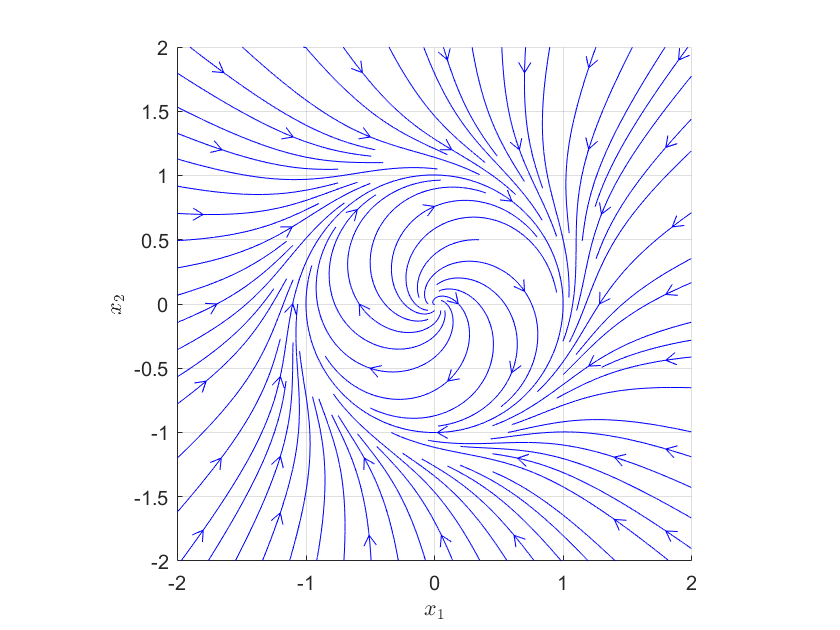
\includegraphics{images/cycle_limite.png}
\caption{Portrait de phase de l'exercice Cycle Limite
I}\label{fig_cycle_limite}
}
\end{figure}

\hypertarget{correc_lyap}{%
\section{Critères de stabilité de Lyapunov}\label{correc_lyap}}

\hypertarget{answer-lyap-1}{%
\subsubsection*{Question 1}\label{answer-lyap-1}}

\addcontentsline{toc}{subsubsection}{Question 1}

Supposons d'abord que \(\langle\nabla V (x), f(x)\rangle \leq 0\) pour
tout \(x\in W\). On a donc pour toute solution \(t\mapsto x(t)\)
initialisée dans \(W\), \(V(x(t))\leq V(x(0))\) tant que \(x(t)\in W\).
Prenons \(\varepsilon>0\) suffisamment petit tel que
\(B_f(a,2\varepsilon)\subset W\). On veut montrer qu'il existe \(\eta\)
tel que toute trajectoire initialisée dans \(B(a,\eta)\) reste dans
\(B(a,\varepsilon)\subset W\). Tout d'abord, il existe
\(\varepsilon_V>0\) tel que \[
\forall x\in B_f(a,2\varepsilon) \ : \ V(x)\leq \varepsilon_V \ \Longrightarrow x\in B(a,\varepsilon) \ .
\] En effet, sinon, il existerait une suite \((x_k)_{k\in \mathbb{N}}\)
d'éléments de \(B_f(a,2\varepsilon)\) telle que pour tout \(k>0\),
\(V(x_k)\leq \frac{1}{k}\) et \(\|x_k-a\|\geq \varepsilon\). L'ensemble
\(B_f(a,2\varepsilon)\) étant compact, on peut en extraire une
sous-suite convergeant vers \(x^\star\) qui vérifie nécessairement
\(V(x^\star)=0\) par continuité de \(V\) et
\(\|x^\star-a\|\geq \varepsilon\), i.e.~\(x^\star \neq a\). Ceci est
impossible par hypothèse. On a donc l'existence de \(\varepsilon_V\).
Maintenant, par continuité de \(V\) en \(a\) et puisque \(V(a)=0\), il
existe aussi \(\eta>0\) tel que \[
x\in B(a,\eta)  \ \Longrightarrow V(x)\leq \varepsilon_V \ .
\] Soit alors une solution maximale \(x\) avec \(x(0)\in B(a,\eta)\).
Attention, la décroissance de \(V(x(t))\) n'est acquise que tant que
\(x(t)\in W\)\,: il faut donc s'assurer que la solution ne quitte pas
\(W\). Supposons par l'absurde que \(x\) sorte de
\(B_f(a,2\varepsilon)\), et notons \[
t_1=\inf\{t\geq 0 \ : \ \|x(t)-a\|> 2\varepsilon\} >0 \ .
\] Sur \([0,t_1]\), \(x(t)\in B_f(a,2\varepsilon)\subset W\), donc
\(V(x(t))\leq V(x(0))\leq \varepsilon_V\) et ainsi
\(x(t)\in B(a,\varepsilon)\)\,; en particulier \(\|x(t_1)-a\|<\varepsilon\),
alors que par continuité et définition de \(t_1\),
\(\|x(t_1)-a\|=2\varepsilon\)~: contradiction. Donc \(x(t)\) reste dans
\(B_f(a,2\varepsilon)\subset W\), et le même argument donne
\(x(t)\in B(a,\varepsilon)\) pour tout \(t\geq 0\) tant qu'elle est
définie. Elle reste ainsi dans un compact de \(X\), donc par le
\protect\hyperlink{theo_bouts}{théorème du domaine maximal d'existence
(p. \pageref*{theo_bouts})}, \(x\) est définie sur
\(\mathbb{R}_{\geq 0}\). Ceci prouve la stabilité de \(a\).

\hypertarget{answer-lyap-2}{%
\subsubsection*{Question 2}\label{answer-lyap-2}}

\addcontentsline{toc}{subsubsection}{Question 2}

Supposons maintenant \(\langle\nabla V (x), f(x)\rangle < 0\) pour tout
\(x\in W\setminus \{a\}\). Alors par le point précédent \(a\) est
stable. Il suffit de montrer l'attractivité locale. Par stabilité, si
\(x(0)\in B(a,\eta)\), \(x(t)\in B(a,\varepsilon)\subset W\) pour tout
\(t\) et \(t\to V(x(t))\) est donc strictement décroissante. Comme elle
est aussi bornée inférieurement par 0, elle converge vers
\(\ell \geq 0\). Supposons \(\ell>0\). Alors, par continuité de \(V\),
il existe \(0<\nu<\varepsilon\) et \(\overline{t}>0\) tel que pour tout
\(t\geq \overline{t}\), \(\|x(t)-a\| \geq \nu\). Soit \[
\gamma = \max_{\nu \leq \|x-a\| \leq \varepsilon} \langle\nabla V (x), f(x)\rangle   
\] qui existe par continuité de \(\nabla V\) et \(f\) sur un compact.
Puisque \(\langle\nabla V (x), f(x)\rangle < 0\) sur
\(W\setminus \{a\}\), \(\gamma<0\). Alors, pour tout
\(t\geq \overline{t}\), \[
V(x(t)) = V(x(\overline{t})) + \int_{\overline{t}}^t \langle\nabla V (x(s)), f(x(s))\rangle ds \leq  V(x(\overline{t})) + \gamma (t-\overline{t}) \ .
\] Mais comme \(\gamma<0\) cette quantité devient strictement négative
au bout d'un certain temps, ce qui est impossible. Donc
\(\lim_{t\to +\infty} V(x(t))=0\). Finalement, reproduisant le même
raisonnement que pour l'existence de \(\varepsilon_V\), on peut garantir
que \(\|x-a\|\) est arbitrairement petit en prenant \(V(x)\)
suffisamment petit. Donc on en déduit que
\(\lim_{t\to +\infty} \|x(t)-a\|=0\).

\hypertarget{answer-lyap-3}{%
\subsubsection*{Question 3}\label{answer-lyap-3}}

\addcontentsline{toc}{subsubsection}{Question 3}

Supposons enfin que \(\lim_{\|x\|\to +\infty} V(x) = +\infty\) et
\(W=\mathbb{R}^n\). Alors \(V(x(t))\leq V(x(0))\) pour tout \(t\in I\), \(t\geq 0\), donc
\(x(t)\in V^{-1}(\left[ 0,V(x(0)) \right])\) pour tout \(t\geq 0\). Le fait
que \(\lim_{\|x\|\to +\infty} V(x) = +\infty\) est équivalent au fait
que l'image réciproque de toute compact est compact (on dit que \(V\)
est propre). Donc \(V^{-1}(\left[ 0,V(x(0)) \right])\) est compact et
par le \protect\hyperlink{theo_bouts}{théorème du domaine maximal
d'existence nécessairement (p. \pageref*{theo_bouts})} \(x(t)\) est
défini pour tout \(t\geq 0\), et reste dans ce compact. Alors on peut
reproduire le même raisonnement que plus haut et obtenir la convergence
de \(x\) vers \(a\).

\hypertarget{answer-lyap-4}{%
\subsubsection*{Question 4 (Application à la stabilité des systèmes
linéaires)}\label{answer-lyap-4}}

\addcontentsline{toc}{subsubsection}{Question 4 (Application à la stabilité des systèmes linéaires)}

Puisque les valeurs propres de \(A\) sont à partie réelle strictement
négative, il existe \(C\geq 1\) et \(\mu>0\) tels que
\(\|e^{As}\|\leq C e^{-\mu s}\) pour tout \(s\geq 0\). L'intégrale \[
P=\int_0^{+\infty}\left(e^{As}\right)^\top Q e^{As}ds
\] est donc bien définie (absolument convergente). La matrice \(P\) est
symétrique car l'intégrande l'est. Pour tout \(x\in\mathbb{R}^n\), \[
x^\top P x = \int_0^{+\infty}\left(e^{As}x\right)^\top Q \left(e^{As}x\right)ds
\geq \lambda_{\min}(Q)\int_0^{+\infty}\|e^{As}x\|^2 ds \ ,
\] qui est strictement positif si \(x\neq 0\) car \(e^{As}\) est
inversible et \(s\mapsto \|e^{As}x\|^2\) est continue. Donc \(P\) est
définie positive. Enfin, puisque \(A\) commute avec \(e^{As}\), \[
A^\top P + PA = \int_0^{+\infty}\left( A^\top e^{A^\top s} Q e^{As} + e^{A^\top s} Q e^{As} A \right) ds
= \int_0^{+\infty}\frac{d}{ds}\left( e^{A^\top s} Q e^{As} \right) ds
= \lim_{S\to+\infty} e^{A^\top S} Q e^{AS} - Q = -Q \ ,
\] car \(\|e^{AS}\|\to 0\) lorsque \(S\to +\infty\).

Posons alors \(V(x)=x^\top P x\). Cette fonction est \(C^1\), \(V(0)=0\),
\(V(x)>0\) pour \(x\neq 0\), et
\(V(x)\geq \lambda_{\min}(P)\|x\|^2\to+\infty\) lorsque
\(\|x\|\to+\infty\). De plus, pour tout \(x\), \[
\langle \nabla V(x), Ax\rangle = 2x^\top P A x = x^\top\left(A^\top P + PA\right)x = -x^\top Q x < 0 \qquad \forall x\neq 0 \ .
\] Par la question 3 (avec \(f(x)=Ax\), \(a=0\), \(W=\mathbb{R}^n\)), \(0\)
est globalement asymptotiquement stable pour \(\dot{x}=Ax\).

\hypertarget{answer-lyap-5}{%
\subsubsection*{Question 5 (Application à la stabilité via linéarisé
tangent)}\label{answer-lyap-5}}

\addcontentsline{toc}{subsubsection}{Question 5 (Application à la stabilité via linéarisé tangent)}

Posons \(J=J_f(a)\) et \[
\Delta(x) = f(x)-f(a) - J(x-a) = f(x)- J(x-a)\ ,
\] puisque \(f(a)=0\). Par différentiabilité de \(f\) en \(a\), la
fonction \(\delta\) définie par \(\delta(x)=\Delta(x)/\|x-a\|\) pour
\(x\neq a\) et \(\delta(a)=0\) vérifie \(\lim_{x\to a}\delta(x)=0\), et
\(\Delta(x)=\delta(x)\|x-a\|\) pour tout \(x\).

Par la question 4 avec \(A=J\) et \(Q=I\), il existe \(P=P^\top>0\) telle
que \[
J^\top P +P J = -I \ .
\] Considérons \(V(x) = (x-a)^\top P (x-a)\), qui est \(C^1\), positive
et nulle seulement en \(x=a\). Pour tout \(x\in X\), \begin{align*}
\left< \nabla V(x), f(x) \right> & = 2(x-a)^\top P f(x) \\
&= (x-a)^\top\left( J^\top P +P J\right) (x-a) + 2 (x-a)^\top P\Delta(x) \\
&\leq - \|x-a\|^2 + 2 \|x-a\| \|P\| \|\Delta(x)\| \\
&\leq - \|x-a\|^2\left(1- 2\|P\|  \|\delta(x) \| \right) \ .
\end{align*} Comme \(X\) est ouvert et \(\delta(x)\to 0\) lorsque
\(x\to a\), il existe \(r>0\) tel que \(B(a,r)\subset X\) et \[
\|\delta(x) \| \leq  \frac{1}{4\|P\|}  \qquad \forall x\in B(a,r) \ .
\] Alors \(\left< \nabla V(x), f(x) \right> \leq -\frac{1}{2}\|x-a\|^2 <0\)
pour tout \(x\in B(a,r)\setminus\{a\}\). Par la question 2 (avec
\(W=B(a,r)\)), \(a\) est localement asymptotiquement stable.

\hypertarget{correc_instab}{%
\section{Critères d'instabilité}\label{correc_instab}}

\hypertarget{answer-instab-1}{%
\subsubsection*{Question 1 (Théorème de Chetaev)}\label{answer-instab-1}}

\addcontentsline{toc}{subsubsection}{Question 1 (Théorème de Chetaev)}

Supposons par l'absurde que \(a\) soit stable. Prenons
\(\varepsilon>0\) tel que \(B_f(a,\varepsilon)\subset W\). Par
stabilité, il existe \(\eta>0\) tel que toute solution maximale
initialisée dans \(B_f(a,\eta)\) est définie sur
\(\mathbb{R}_{\geq 0}\) et reste dans \(B_f(a,\varepsilon)\). Par
hypothèse, il existe \(x_0\in B(a,\eta)\) tel que \(V(x_0)>0\). Soit
\(x\) une solution maximale initialisée en \(x_0\) et
\(v(t)=V(x(t))\), qui est \(C^1\) sur \(\mathbb{R}_{\geq 0}\) avec \[
\dot{v}(t) = \langle\nabla V (x(t)), f(x(t))\rangle \ .
\] Montrons d'abord que \(v(t)\geq v(0)\) pour tout \(t\geq 0\). Sinon,
\(t_1 = \inf\{t\geq 0 \ : \ v(t)<v(0)\}\) vérifie \(v(t_1)=v(0)>0\) par
continuité, donc \(\dot{v}(t_1)>0\) par hypothèse, et \(v>v(0)\) sur un
intervalle \(]t_1,t_1+h]\), ce qui contredit la définition de \(t_1\).
Ainsi, pour tout \(t\geq 0\), \(x(t)\) appartient à \[
K = \left\{ x\in B_f(a,\varepsilon) \ : \ V(x)\geq V(x_0) \right\} \ ,
\] qui est compact (fermé dans le compact \(B_f(a,\varepsilon)\) par
continuité de \(V\)) et ne contient pas \(a\) puisque \(V(a)=0<V(x_0)\).
Soit \[
\gamma = \min_{x\in K} \langle\nabla V (x), f(x)\rangle
\] qui existe par continuité de \(\nabla V\) et \(f\) sur le compact
\(K\). Puisque \(V>0\) sur \(K\), \(\gamma>0\) par hypothèse. Alors,
pour tout \(t\geq 0\), \[
V(x(t)) = V(x_0) + \int_0^t \langle\nabla V (x(s)), f(x(s))\rangle ds \geq V(x_0) + \gamma t \ ,
\] qui tend vers \(+\infty\). C'est impossible puisque \(V\) est
continue donc bornée sur le compact \(B_f(a,\varepsilon)\). Donc \(a\)
est instable.

\hypertarget{answer-instab-2}{%
\subsubsection*{Question 2 (Exemples)}\label{answer-instab-2}}

\addcontentsline{toc}{subsubsection}{Question 2 (Exemples)}

Pour \(\dot{x}=x^3\), prenons \(V(x)=x^2\), qui est \(C^1\), nulle en
\(0\) et strictement positive ailleurs. On a
\(\langle\nabla V (x), x^3\rangle = 2x^4 >0\) pour tout \(x\neq 0\), donc
\(0\) est instable par la question 1 avec \(W=\mathbb{R}\). Notons que
le \protect\hyperlink{theo_linTangent}{théorème du linéarisé tangent (p.
\pageref*{theo_linTangent})} ne permet pas de conclure ici puisque le
linéarisé en \(0\) est nul. On peut d'ailleurs vérifier que la solution
initialisée en \(x_0\neq 0\) est
\(x(t)=\frac{x_0}{\sqrt{1-2x_0^2 t}}\), qui explose en temps fini
\(t=\frac{1}{2x_0^2}\), aussi proche de \(0\) que soit \(x_0\).

Pour le second système, prenons \(V(x)=x_1^2-x_2^2\), qui n'est pas de
signe constant. On a \(V(0)=0\), \(V(\eta,0)=\eta^2>0\) pour tout
\(\eta>0\), et \[
\langle\nabla V (x), f(x)\rangle = 2x_1\cdot x_1 - 2x_2\cdot(-x_2) = 2\|x\|^2 >0 \qquad \forall x\neq 0 \ ,
\] en particulier lorsque \(V(x)>0\). Par la question 1 avec
\(W=\mathbb{R}^2\), \(0\) est instable. Les trajectoires s'éloignent en
effet de \(0\) selon la direction \(x_1\)~: c'est un \emph{point selle}.

\hypertarget{answer-instab-3}{%
\subsubsection*{Question 3 (Application à l'instabilité des systèmes
linéaires)}\label{answer-instab-3}}

\addcontentsline{toc}{subsubsection}{Question 3 (Application à l'instabilité des systèmes linéaires)}

Notons \(\lambda_1,\ldots,\lambda_p\) les valeurs propres (complexes,
distinctes) de \(A\), de multiplicités \(m_1,\ldots,m_p\), et
\(\mu = \max_i \mathrm{Re}(\lambda_i)>0\). Choisissons
\(\sigma\in \, ]0,\mu[\) différent de tous les \(\mathrm{Re}(\lambda_i)\),
ce qui est possible puisqu'ils sont en nombre fini. Ce décalage permet
de traiter les éventuelles valeurs propres de partie réelle nulle, qui
ne sont ni \og stables\fg{} ni \og instables\fg{}~: elles sont ici rangées
du côté stable.

Écrivons le polynôme caractéristique \(\chi_A=\chi_+\chi_-\), où
\(\chi_+\) (resp. \(\chi_-\)) est le produit des facteurs
\((X-\lambda_i)^{m_i}\) tels que \(\mathrm{Re}(\lambda_i)>\sigma\) (resp.
\(\mathrm{Re}(\lambda_i)<\sigma\)). Les valeurs propres non réelles de
\(A\) étant deux à deux conjuguées avec la même multiplicité, \(\chi_+\)
et \(\chi_-\) sont à coefficients réels, et ils sont premiers entre eux.
Par le théorème de Cayley-Hamilton et le lemme des noyaux, \[
\mathbb{R}^n = E_+ \oplus E_- \qquad , \qquad E_\pm = \ker \chi_\pm(A) \ ,
\] où \(E_+\) et \(E_-\) (éventuellement réduit à \(\{0\}\)) sont stables
par \(A\). Il existe donc \(T\in \mathbb{R}^{n\times n}\) inversible
(dont les colonnes sont une base de \(E_+\) suivie d'une base de
\(E_-\)) telle que \[
T^{-1}AT = \left( \begin{matrix} A_+ & 0\\ 0 & A_- \end{matrix}\right) \ ,
\] où \(\chi_\pm(A_\pm)=0\). Les valeurs propres de \(A_+\) sont donc des
racines de \(\chi_+\), c'est-à-dire de partie réelle \(>\sigma\), et
celles de \(A_-\) sont de partie réelle \(<\sigma\). Par ailleurs,
\(E_+\neq\{0\}\)~: si \(v\in\mathbb{C}^n\) est un vecteur propre associé
à une valeur propre \(\lambda\) de partie réelle \(\mu\), alors
\(\chi_+(A)v = \chi_+(\lambda)v = 0\), donc \(\mathrm{Re}(v)\) et
\(\mathrm{Im}(v)\), qui ne sont pas tous deux nuls, sont dans \(E_+\)
puisque \(\chi_+(A)\) est réelle.

Les valeurs propres de \(\sigma I-A_+\) et de \(A_- - \sigma I\) sont
donc toutes à partie réelle strictement négative. Par la
\protect\hyperlink{lyap-4}{question 4 de l'exercice \emph{Critères de
stabilité de Lyapunov} (p. \pageref*{lyap-4})} appliquée avec
\(Q=I\), il existe \(P_+\) et \(P_-\) symétriques définies positives
telles que \[
(\sigma I-A_+)^\top P_+ + P_+(\sigma I-A_+) = -I \qquad , \qquad (A_- -\sigma I)^\top P_- + P_-(A_- -\sigma I) = -I \ ,
\] c'est-à-dire \[
A_+^\top P_+ + P_+A_+ = 2\sigma P_+ + I \qquad , \qquad A_-^\top P_- + P_-A_- = 2\sigma P_- - I \ .
\] Posons alors, avec \(T^{-\top}=(T^{-1})^\top\), \[
D = \left( \begin{matrix} P_+ & 0\\ 0 & -P_- \end{matrix}\right) \qquad , \qquad P = T^{-\top} D\, T^{-1} \qquad , \qquad Q = T^{-\top} T^{-1} \ .
\] Les matrices \(P\) et \(Q\) sont symétriques, \(Q\) est définie
positive, et en notant \(M=T^{-1}AT\), \begin{align*}
A^\top P + PA &= T^{-\top}\left( M^\top D + D M\right) T^{-1} \\
&= T^{-\top} \left( \begin{matrix} A_+^\top P_+ + P_+A_+ & 0\\ 0 & -(A_-^\top P_- + P_-A_-) \end{matrix}\right) T^{-1} \\
&= T^{-\top} \left( 2\sigma D + I \right) T^{-1} = 2\sigma P + Q \ .
\end{align*} Enfin, pour \(z_+\in\mathbb{R}^{\dim E_+}\) non nul et
\(\bar{x} = T(z_+,0)\), on a \(\bar{x}^\top P \bar{x} = z_+^\top P_+ z_+>0\).

Considérons maintenant \(V(x)=x^\top P x\). On a \(V(0)=0\) et, pour
tout \(t>0\), \(V(t\bar{x}) = t^2\,\bar{x}^\top P \bar{x}>0\), donc
\(V\) prend des valeurs strictement positives arbitrairement près de
\(0\). De plus, pour tout \(x\in\mathbb{R}^n\), \[
\langle\nabla V (x), Ax\rangle = 2x^\top PAx = x^\top\left(A^\top P + PA\right) x = 2\sigma V(x) + x^\top Q x \ ,
\] qui est strictement positif dès que \(V(x)>0\) (et donc
\(x\neq 0\)). Par la question 1 avec \(W=\mathbb{R}^n\), \(0\) est
instable pour \(\dot{x}=Ax\).

Notons que pour un système linéaire, on pouvait conclure plus
directement~: si \(v\) est un vecteur propre associé à une valeur propre
\(\lambda\) de partie réelle strictement positive, la solution
initialisée en \(\eta\,\mathrm{Re}(v)\) s'écrit
\(x(t)=\eta\,\mathrm{Re}(e^{\lambda t}v)\) et n'est pas bornée, aussi
petit que soit \(\eta>0\). L'intérêt de la fonction \(V\) construite
ici est qu'elle reste une fonction de Chetaev pour des perturbations non
linéaires de \(\dot{x}=Ax\), comme on va le voir à la question suivante.

\hypertarget{answer-instab-4}{%
\subsubsection*{Question 4 (Application à l'instabilité via linéarisé
tangent)}\label{answer-instab-4}}

\addcontentsline{toc}{subsubsection}{Question 4 (Application à l'instabilité via linéarisé tangent)}

Comme dans la \protect\hyperlink{answer-lyap-5}{question 5 de l'exercice
\emph{Critères de stabilité de Lyapunov} (p. \pageref*{answer-lyap-5})},
posons \(J=J_f(a)\) et \(\Delta(x) = f(x) - J(x-a)\), de sorte que
\(\Delta(x)=\delta(x)\|x-a\|\) avec \(\lim_{x\to a}\delta(x)=0\). Par la
question 3 appliquée à \(A=J\), il existe \(\sigma>0\), \(Q\) symétrique
définie positive et \(P\) symétrique telles que \[
J^\top P + PJ = 2\sigma P + Q \ ,
\] et \(\bar{x}\in\mathbb{R}^n\) tel que \(\bar{x}^\top P \bar{x}>0\)
(en particulier \(P\neq 0\)). Considérons
\(V(x) = (x-a)^\top P (x-a)\). Pour tout \(x\in X\), \begin{align*}
\left< \nabla V(x), f(x) \right> & = 2(x-a)^\top P f(x) \\
&= (x-a)^\top\left( J^\top P +P J\right) (x-a) + 2 (x-a)^\top P\Delta(x) \\
&= 2\sigma V(x) + (x-a)^\top Q (x-a) + 2 (x-a)^\top P\Delta(x) \\
&\geq 2\sigma V(x) + \lambda_{\min}(Q)\|x-a\|^2 - 2 \|P\|  \|\delta(x) \| \|x-a\|^2 \ .
\end{align*} Comme \(X\) est ouvert et \(\delta(x)\to 0\) lorsque
\(x\to a\), il existe \(r>0\) tel que \(B(a,r)\subset X\) et \[
\|\delta(x) \| \leq  \frac{\lambda_{\min}(Q)}{4\|P\|}  \qquad \forall x\in B(a,r) \ .
\] Alors, pour tout \(x\in B(a,r)\), \[
\left< \nabla V(x), f(x) \right> \geq 2\sigma V(x) + \frac{\lambda_{\min}(Q)}{2}\|x-a\|^2 \ ,
\] qui est strictement positif dès que \(V(x)>0\) (et donc \(x\neq a\)).
Par ailleurs \(V(a)=0\) et \(V(a+t\bar{x}) = t^2\,\bar{x}^\top P \bar{x}>0\)
pour tout \(t>0\), avec \(a+t\bar{x}\in B(a,r)\) pour \(t\) assez
petit. Par la question 1 avec \(W=B(a,r)\), \(a\) est instable.

\hypertarget{correc_cycle_lim_volterra}{%
\section{Cycle limite II}\label{correc_cycle_lim_volterra}}

On étudie le comportement des solutions de \(\dot{x}=f(x)\) pour \[
f(x) = 
\left(
\begin{matrix}
x_1(\alpha -\beta x_2)  \\
-x_2(\gamma-\delta x_1)
\end{matrix}
\right)
\]

\hypertarget{answer-cycle-lim-volterra-1}{%
\subsubsection*{Question 1}\label{answer-cycle-lim-volterra-1}}

\addcontentsline{toc}{subsubsection}{Question 1}

On résout \(f(x) = 0\), ce qui donne les points d'équilibre \((0,0)\) et
\(\bar{x}=\left(\frac{\gamma}{\delta},\frac{\alpha}{\beta} \right)\).

La jacobienne de la dynamique est donnée par \[
J_f(x) = 
\left(
\begin{matrix}
\alpha -\beta x_2 & -\beta x_1 \\
\delta x_2 & -(\gamma-\delta x_1)
\end{matrix}
\right)
\] En \((0,0)\), \[
J_f(0,0) = 
\left(
\begin{matrix}
\alpha & 0 \\
0 & -\gamma
\end{matrix}
\right)
\] a pour valeur propre \(\alpha>0\), donc \((0,0)\) est instable. Par
contre, en \(\bar{x}\), \[
J_f(\bar{x}) = 
\left(
\begin{matrix}
0 & -\beta\frac{\gamma}{\delta} \\
\delta\frac{\alpha}{\beta} & 0
\end{matrix}
\right)
\] a des valeurs propres imaginaires pures \(\pm i\sqrt{\alpha\gamma}\),
donc a priori on ne peut rien dire sur la stabilité de \(\bar{x}\) pour le système
non linéaire.

\hypertarget{answer-cycle-lim-volterra-2}{%
\subsubsection*{Question 2}\label{answer-cycle-lim-volterra-2}}

\addcontentsline{toc}{subsubsection}{Question 2}

Soit \(x_0=(0,x_{2,0})\in \{0\}\times \mathbb{R}_{\geq 0}\) sur l'axe
des ordonnées. Puisque \(f\) est \(C^1\) sur \(\mathbb{R}^2\), par le
théorème de Cauchy-Lipschitz, le problème de Cauchy associé à la
condition initiale \((t_0,x_0)\) pour un \(t_0\) quelconque, admet une
unique solution \[
x(t) = (0, x_2(t))
\] définie sur \(\mathbb{R}\) avec \(x_2\) solution de \[
\dot{x}_2 = -\gamma x_2 \ .
\]

De même, pour \(x_0=(x_{1,0},0)\in \mathbb{R}_{\geq 0}\times \{0\}\), le
problème de Cauchy associé pour un \(t_0\) quelconque, admet une unique
solution du type \[
x(t) = (x_1(t), 0)
\] définie sur \(\mathbb{R}\) avec \(x_1\) solution de \[
\dot{x}_1 = \alpha x_1 \ .
\]

Si une solution initialisée dans
\(\mathbb{R}_{>0}\times\mathbb{R}_{>0}\) croisait l'axe des abscisses ou
des ordonnées, il existerait une autre solution au problème de Cauchy
associé à \(x_0=(0,x_{2,0})\) ou \(x_0=(x_{1,0},0)\) qui ne resterait
pas sur l'axe en temps négatif, ce qui est impossible. Elle reste donc
dans \(\mathbb{R}_{>0}\times\mathbb{R}_{>0}\).

\hypertarget{answer-cycle-lim-volterra-3}{%
\subsubsection*{Question 3}\label{answer-cycle-lim-volterra-3}}

\addcontentsline{toc}{subsubsection}{Question 3}

\(f\) est continue sur \(\mathbb{R}^2\) donc d'après le
théorème du domaine maximal d'existence, si une solution maximale
initialisée dans \(\mathbb{R}^2\) n'est pas définie sur
\(\mathbb{R}\), c'est que nécessairement \(\|x\|\) diverge en temps fini
(car la frontière de \(\mathbb{R}^2\) est vide).

Maintenant considérons une solution maximale
\(x:I\subset \mathbb{R} \to \mathbb{R}^2\) initialisée dans
\(\mathbb{R}_{>0}\times\mathbb{R}_{>0}\). Par la question précédente,
elle reste dans \(\mathbb{R}_{>0}\times\mathbb{R}_{>0}\) donc
\(H(x(t))\) est bien définie pour tout \(t\in I\), et on a \[
\frac{d}{dt}H(x(t)) = \langle \nabla H(x(t)) , \dot{x}(t) \rangle =  \langle \nabla H(x(t)) , f(x(t)) \rangle =0
\] Donc \(H\) est constante et il est impossible que \(\|x\|\) diverge
en temps fini car on aurait \(\lim H(x(t)) = +\infty\). Donc
\(I=\mathbb{R}\).

\emph{Remarque}~: On aurait pu aussi directement se placer sur
\(\mathbb{R}_{>0}\times\mathbb{R}_{>0}\) et considérer les solutions
maximales
\(x:I\subset \mathbb{R} \to \mathbb{R}_{>0}\times\mathbb{R}_{>0}\) de
\(\dot{x}=f(x)\) dans cet ensemble (où \(f\) est bien sûr continue). Si
\(x\) n'était pas définie sur \(\mathbb{R}\), alors nécessairement
d'après le théorème du domaine maximal d'existence, \(x(t)\) finirait,
en temps fini, par être à chaque instant soit arbitrairement loin de
l'origine, soit arbitrairement proche de la frontière de
\(\mathbb{R}_{>0}\times\mathbb{R}_{>0}\), c'est-à-dire avec \(x_1\) ou
\(x_2\) arbitrairement petit. Mais ceci est impossible car
\(H(x) = u_{\delta,\gamma}(x_1) + u_{\beta,\alpha}(x_2)\), où
\(u_{c,d}(z) = cz - d\ln z\) est minorée et tend vers \(+\infty\) en
\(0^+\) comme en \(+\infty\)~: dans chacun des cas on aurait \[
\lim H(x(t)) = +\infty \ ,
\] contredisant la conservation de \(H\). On prouve alors en même temps que les solutions initialisées dans
\(\mathbb{R}_{>0}\times\mathbb{R}_{>0}\) sont définies sur
\(\mathbb{R}\) dans \(\mathbb{R}_{>0}\times\mathbb{R}_{>0}\) (et donc
restent dans cet ensemble)

\emph{Bonus}~: Ici, en calculant le gradient et la hessienne de \(H\)
(voir Calcul Différentiel III), on voit que \(H\) atteint un minimum
local (et en fait global) en \(\bar{x}\) (gradient nul et matrice
hessienne définie positive, mais on peut aussi le montrer en étudiant la
fonction réelle \(u(z)=z-c\ln z\) pour une constante \(c>0\)). Donc
\[
V(x) = H(x)-H(\bar{x})
\] est une fonction \(C^1\) sur
\(\mathbb{R}_{>0}\times\mathbb{R}_{>0}\), positive, qui ne s'annule
localement qu'en \(\bar{x}\). Vu que \(H\) est conservée le long des
trajectoires, on peut déduire que \(\bar{x}\) est stable par le
\protect\hyperlink{stab_decroissance}{théorème de décroissance (p.
\pageref*{stab_decroissance})}.

\hypertarget{answer-cycle-lim-volterra-4}{%
\subsubsection*{Question 4}\label{answer-cycle-lim-volterra-4}}

\addcontentsline{toc}{subsubsection}{Question 4}

L'équilibre \(\bar{x}\) se trouve au milieu des courbes de niveau (car
c'est en fait le minimum de \(H\)). Donc si on se donne
\(\varepsilon >0\), on peut trouver \(\eta_H>0\) tel que \(H(x)-H(\bar{x})<\eta_H\)
implique \(\|x-\bar{x}\|<\varepsilon\). On en déduit que pour toute
condition initiale telle que \(H(x_0)-H(\bar{x})<\eta_H\), la trajectoire reste à
une distance inférieure à \(\varepsilon\) de \(\bar{x}\). Par ailleurs,
l'ensemble des courbes de niveau de \(H-H(\bar{x})\) inférieures à \(\eta_H\)
constituent bien un voisinage de \(\bar{x}\) donc \(\bar{x}\) est stable
par définition.

Le portrait de phase est donné
\protect\hyperlink{fig_cycle_limiteII}{Figure~\ref*{fig_cycle_limiteII} (p.
\pageref*{fig_cycle_limiteII})}.

\begin{figure}
\hypertarget{fig_cycle_limiteII}{%
\centering
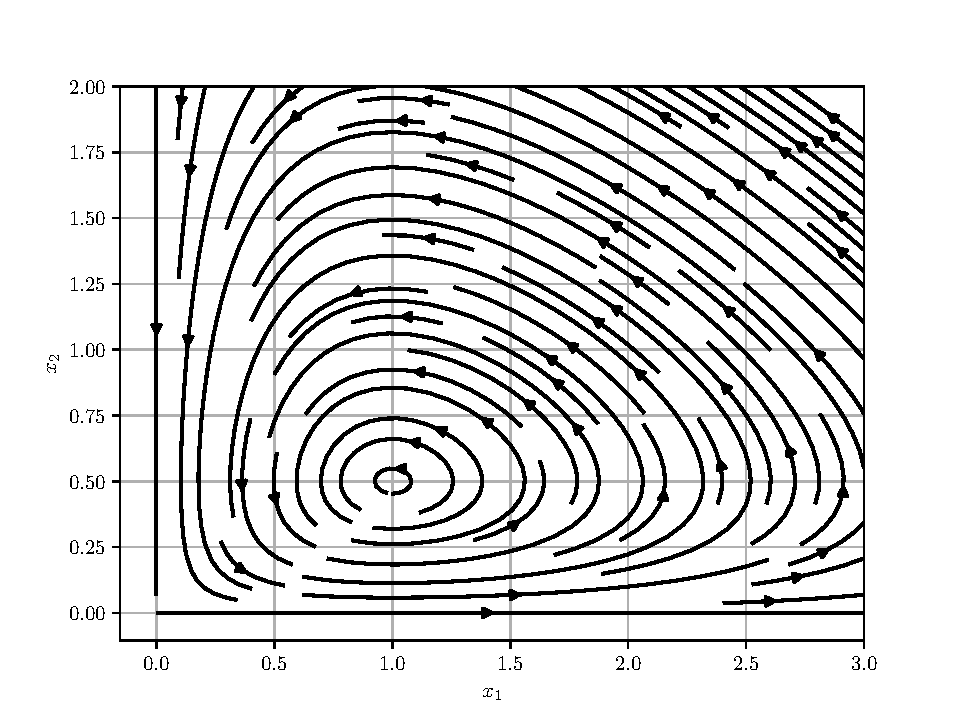
\includegraphics{images/cycle_limiteII.py.pdf}
\caption{Portrait de phase de l'exercice Cycle Limite
II}\label{fig_cycle_limiteII}
}
\end{figure}

\hypertarget{answer-cycle-lim-volterra-5}{%
\subsubsection*{Question 5}\label{answer-cycle-lim-volterra-5}}

\addcontentsline{toc}{subsubsection}{Question 5}

Pour que \(x_1\) vale \(x_1^*\) à l'équilibre, il faut que \(x_2\) vale
\(x_2^* = \frac{\alpha}{\beta}\) et
\(u^* = x_2^*(\gamma-\delta x_1^*)\).

\hypertarget{answer-cycle-lim-volterra-6}{%
\subsubsection*{Question 6}\label{answer-cycle-lim-volterra-6}}

\addcontentsline{toc}{subsubsection}{Question 6}

Commençons par justifier le choix de la référence \(v_r\). Si l'on
parvenait à imposer \(x_2 = v_r(x_1)\), la première équation deviendrait
\[
\dot{x}_1 = x_1\big(\alpha - \beta v_r(x_1)\big) = -\beta\lambda_1\, x_1 (x_1-x_1^*) \ ,
\] équation scalaire pour laquelle \(x_1^*\) est asymptotiquement stable
sur \(\mathbb{R}_{>0}\) (\(\dot{x}_1<0\) si \(x_1>x_1^*\), \(\dot{x}_1>0\)
si \(0<x_1<x_1^*\)). La référence \(v_r(x_1)=\frac{\alpha}{\beta}+\lambda_1(x_1-x_1^*)\)
corrige donc la valeur d'équilibre \(\frac{\alpha}{\beta}\) des
prédateurs proportionnellement à l'écart des proies à leur cible\,:
plus de prédateurs s'il y a trop de proies, moins s'il n'y en a pas
assez. Il reste à faire converger \(x_2\) vers \(v_r(x_1)\) à l'aide de
\(u\), ce que mesure le second terme de \(V\).

On utilise ici pour simplifier le deuxième
\protect\hyperlink{exo_lyap}{critère de Lyapunov (p.
\pageref*{exo_lyap})}. La fonction \(V\) est \(C^1\), à valeurs
positives et s'annule si et seulement si \(x_1=x_1^*\) et
\(x_2 = v_r(x_1^*)=x_2^*\). C'est donc une fonction de Lyapunov associée à
\((x_1^*,x_2^*)\). Calculons sa dérivée le long des trajectoires.
\begin{multline*}
\langle \nabla V(x) , f(x) \rangle = -2\beta\lambda_1 x_1(x_1-x_1^*)^2 -2\beta x_1(x_1-x_1^*)(x_2-v_r(x_1)) \\
+ 2(x_2-v_r(x_1))\left(-x_2(\gamma-\delta x_1)+u - \lambda_1 f_1(x) \right)
\end{multline*} en utilisant \(\alpha-\beta x_2 = -\beta\lambda_1(x_1-x_1^*) - \beta(x_2-v_r(x_1))\)
et \(\frac{d}{dt}\left(x_2-v_r(x_1)\right) = \dot{x}_2 - v_r'(x_1)\dot{x}_1 = \dot{x}_2 - \lambda_1 f_1(x)\).
L'idée est alors de choisir \(u\) afin d'assurer que
\(\langle \nabla V(x) , f(x) \rangle< 0\) au moins dans un voisinage de
l'équilibre. On prend donc par exemple \[
u =  -\lambda_2(x_2-v_r(x_1)) + x_2(\gamma-\delta x_1) + \lambda_1f_1(x) + \beta x_1(x_1-x_1^*)
\] avec \(\lambda_2>0\). Ceci donne \[
\langle \nabla V(x) , f(x) \rangle = -2\beta\lambda_1 x_1(x_1-x_1^*)^2 -2\lambda_2(x_2-v_r(x_1))^2
\] qui est bien strictement négatif pour \(x\neq (x_1^*,x_2^*)\) dans un
voisinage où \(x_1>0\). On en déduit que \((x_1^*,x_2^*)\) est
localement asymptotiquement stable. Il ne l'est pas globalement car
\((0,v_r(0))=(0,\frac{\alpha}{\beta}-\lambda_1 x_1^*)\) est aussi point d'équilibre
du système bouclé (en \(x_1=0\), on a \(\dot x_2 = -\lambda_2(x_2-v_r(0))\)). Mais ce dernier est instable
(\(\frac{\partial f_1}{\partial x_1}(0,v_r(0)) = \beta\lambda_1 x_1^*>0\))
et une étude plus fine pourrait montrer que le bassin d'attraction
inclut \(\mathbb{R}_{> 0}\times\mathbb{R}_{> 0}\).

\begin{figure}
\hypertarget{fig_cycle_limiteII_control}{%
\centering
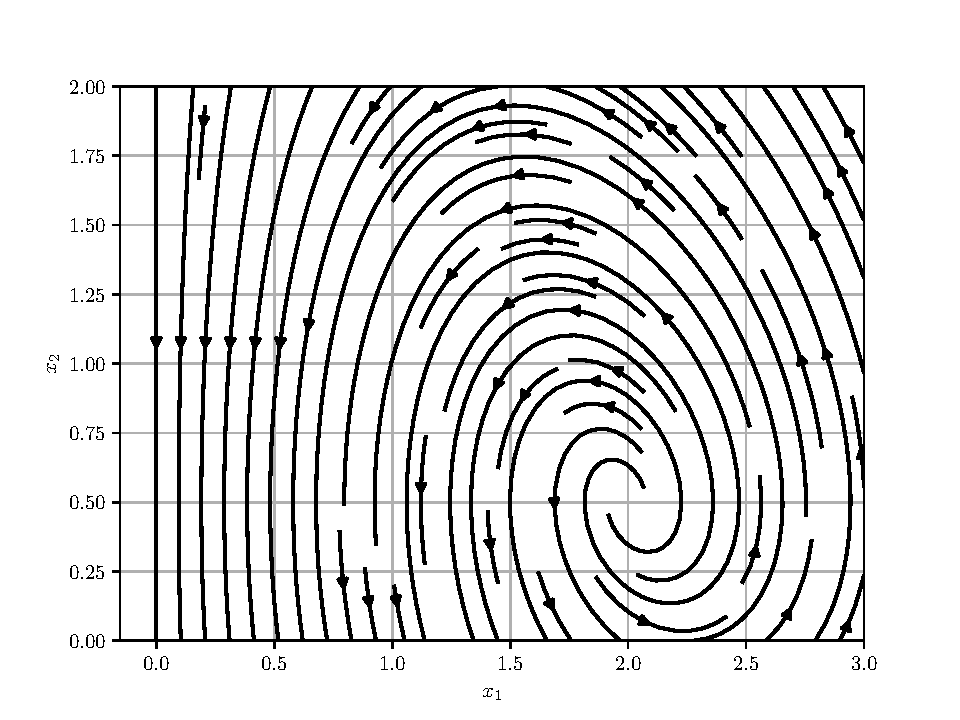
\includegraphics{images/cycle_limiteII_control.py.pdf}
\caption{Portrait de phase de l'exercice Cycle Limite II avec l'entrée
\(u\) choisie pour \(x_1^*=2\) avec
\(\lambda_1=\lambda_2=1\).}\label{fig_cycle_limiteII_control}
}
\end{figure}

\hypertarget{answer-attrac_stab}{%
\section{Attractivité locale implique stabilité asymptotique globale
pour un système linéaire}\label{answer-attrac_stab}}

Tout d'abord, montrons que l'attractivité locale de 0 implique
l'attractivité globale. Ceci est dû à la propriété d'\emph{homogénéité}
des systèmes linéaires: si \(x\) est une solution initialisée à
\(x_0\in\mathbb{R}\), alors \(\lambda x\) est solution initialisée à
\(\lambda x_0\) puisque \[
\lambda x(t) = \lambda e^{At} x_0 = e^{At} (\lambda x_0) \ .
\] Donc soit \(\eta>0\) tel que toute solution initialisée dans
\(B(0,\eta)\) converge vers 0. Soit \(x\) une solution initialisée à
\(x_0\in\mathbb{R}\). Alors \(\lambda x\) avec
\(\lambda < \eta / \|x_0\|\) est solution initialisée dans \(B(0,\eta)\)
et converge vers 0. Donc \(x\) converge vers 0.

Maintenant, montrons la stabilité. Soit \(\varepsilon >0\). Notons
\((x_i)_{i=1...n}\) une base orthonormale de \(\mathbb{R}^n\). Soit
alors \(M>0\) tel que \[
\|e^{At} x_i \| \leq M \quad \forall t \in \mathbb{R}_{\geq 0}\quad \forall i\in \{1,...,n\}
\] qui existe bien puisque toutes les solutions convergent vers 0 et
\(n\) est fini. Soit maintenant \(\eta >0\). Pour tout
\(x_0 \in B(0,\eta)\) dont la décomposition dans la base s'écrit \[
x_0 = \sum_{i=1}^n \alpha_i x_i
\] on a \(|\alpha_i|\leq \eta\) et donc pour tout
\(t \in \mathbb{R}_{\geq 0}\), \[
\left\| e^{At} x_0 \right\| \leq \left\| \sum_{i=1}^n  e^{At} \alpha_i x_i\right\|  \leq  n \eta M
\] On conclut que pour des conditions initiales suffisamment petites
(\(\eta <\frac{\varepsilon}{nM}\)), les solutions restent inférieures à
\(\varepsilon\) en norme. Donc le système est stable.

\hypertarget{correc_cont_lin}{%
\section{Stabilisation d'une chaîne
d'intégrateurs}\label{correc_cont_lin}}

La dynamique du système est de la forme \(\dot{x} = f(x,u)\).

\hypertarget{answer-cont-lin-1}{%
\subsubsection*{Question 1}\label{answer-cont-lin-1}}

\addcontentsline{toc}{subsubsection}{Question 1}

Pour que \(x^*\) soit point d'équilibre avec la commande \(u^*\), il
faut \(f(x^*,u^*)=0\), soit \(x_2^*=x_3^*=\ldots=x_n^*=0\) et
\(u^* = -\phi(x_1^*,0,\ldots,0)\).

\hypertarget{answer-cont-lin-2}{%
\subsubsection*{Question 2}\label{answer-cont-lin-2}}

\addcontentsline{toc}{subsubsection}{Question 2}

L'idée est de se placer autour de \(x^*\) et donc considérer l'erreur
\(e = x-x^*\) que l'on souhaite stabiliser à 0. On constate alors que \[
\begin{array}{rcl}
\dot{e}_1 &=& e_2 \\
\dot{e}_2 &=& e_3 \\
&\vdots&\\
\dot{e}_{n-1} &=& e_n \\
\dot{e}_n &=& \phi(x) + u(t)
\end{array}
\] Si l'on mesure \(x(t)\), on peut prendre \[
u(t) = -\phi(x(t)) -k_1 e_1(t) - k_2 e_2(t) - \ldots - k_n e_n(t)
\] ce qui donne \[
\dot{e} = A e
\] avec \(A\) de la forme \[
A = \left(
\begin{array}{ccccc}
0&1&0 & \ldots & 0 \\
\vdots &\ddots & \ddots & & \vdots\\
\vdots&&\ddots & 1  &0\\
0&&&0&1 \\
-k_1 &-k_2&\ldots& \ldots& -k_n
\end{array}
\right)
\] qui admet pour polynôme caractéristique \[
s^n + k_n s^{n-1} + \ldots + k_2 s + k_1\ .
\] Il suffit donc de choisir les coefficients \(k_i\) tels que ce
polynôme ait ses racines à partie réelle strictement négative pour que
\(e=0\) soit globalement asymptotiquement stable. En d'autres termes, on
prend \[
u(t) = -\phi(x(t)) -k_1 (x_1(t)-x_1^*) - k_2 x_2(t) - \ldots - k_n x_n(t)
\] c'est-à-dire on corrige le système en fonction de la distance à
\(x^*\). Il s'agit d'un feedback, ou retour d'état en français.

\hypertarget{answer-cont-lin-3}{%
\subsubsection*{Question 3}\label{answer-cont-lin-3}}

\addcontentsline{toc}{subsubsection}{Question 3}

Si l'on voulait stabiliser une trajectoire \(t\mapsto x_r(t)\), il
faudrait d'abord que cette trajectoire soit admissible, c'est-à-dire,
qu'elle soit solution de \(\dot{x}_r=f(x_r,u_r)\) pour une certaine
commande de référence \(u_r\). Dans ce cas, on remarque que
\(e = x-x_r\) vérifie \[
\begin{array}{rcl}
\dot{e}_1 &=& e_2 \\
\dot{e}_2 &=& e_3 \\
&\vdots&\\
\dot{e}_{n-1} &=& e_n \\
\dot{e}_n &=& \phi(x) + u(t) - \dot x_{r,n}
\end{array}
\] et donc similairement, on prendrait \[
u(t) = \dot x_{r,n}-\phi(x(t)) -k_1 (x_1(t)-x_{r,1}(t)) - k_2 (x_2(t) -x_{r,2}(t)) - \ldots - k_n (x_n(t)-x_{r,n}(t)) \ .
\]


\hypertarget{correc_kepler}{%
\section{Problème de Kepler~: collision, libération et orbites
circulaires}\label{correc_kepler}}

\hypertarget{answer-kepler-1}{%
\subsubsection*{Question 1 (Cadre)}\label{answer-kepler-1}}

\addcontentsline{toc}{subsubsection}{Question 1 (Cadre)}

Le système s'écrit \(\dot x = f(x)\) avec \[
f(q,v) = \left(v \,,\, -\mu\frac{q}{\|q\|^3}\right)
\] qui est de classe \(C^\infty\) (donc continûment différentiable, donc
localement lipschitzienne) sur l'ouvert \(X\) puisque \(q\neq 0\) sur
\(X\). Le \protect\hyperlink{theo_lips}{théorème de Cauchy-Lipschitz (p.
\pageref*{theo_lips})} dans sa version localement lipschitzienne donne
l'existence et l'unicité d'une solution maximale pour toute condition
initiale dans \(X\), définie sur un intervalle ouvert
\(\left]\tmin,\tmax\right[\).

Le long d'une solution, \[
\dot E = v\cdot \dot v + \mu\frac{q\cdot \dot q}{\|q\|^3} = -\mu\frac{v\cdot q}{\|q\|^3} + \mu\frac{q\cdot v}{\|q\|^3} = 0
\] en utilisant \(\frac{d}{dt}\|q\| = \frac{q\cdot\dot q}{\|q\|}\), et
\[
\dot L = \dot q\times v + q\times \dot v = v\times v - \frac{\mu}{\|q\|^3}\, q\times q = 0 \ .
\] \(E\) et \(L\) sont donc des \emph{intégrales premières}~: ce sont
les lois de conservation de l'énergie et du moment cinétique.

Ici \(J=\mathbb{R}\) n'a pas de bord et le bord de \(X\) est
\(\partial X = \{0\}\times \mathbb{R}^3\), de sorte que
\(d\big((t,x(t)),\partial(J\times X)\big) = \|q(t)\|\). Le théorème du
domaine maximal dit donc que si \(\tmax<+\infty\), alors \[
\lim_{t\to\tmax} \|(q(t),v(t))\| + \frac{1}{\|q(t)\|} = +\infty \ ,
\] c'est-à-dire qu'à chaque instant proche de \(\tmax\), ou bien
\(\|q(t)\|\) est très petit, le satellite \emph{s'approche du corps
central} (collision), ou bien \(\|(q(t),v(t))\|\) est très grand, la
position ou la vitesse \emph{explosent}. L'existence de
solutions sur \(\mathbb{R}\) entier n'a donc rien d'évident a priori~:
le critère de croissance affine ne s'applique pas, et \(f\) n'est même
pas définie sur \(\mathbb{R}^6\) entier.

\hypertarget{answer-kepler-2}{%
\subsubsection*{Question 2 (Confinement et vitesse de
libération)}\label{answer-kepler-2}}

\addcontentsline{toc}{subsubsection}{Question 2 (Confinement et vitesse de libération)}

Posons \(\rho(t) = \frac{1}{2}\|q(t)\|^2\). On a \(\dot\rho = q\cdot v\)
et \[
\ddot \rho = \|v\|^2 + q\cdot \dot v = \|v\|^2 - \mu\frac{\|q\|^2}{\|q\|^3} = \|v\|^2 - \frac{\mu}{\|q\|} = 2E + \frac{\mu}{\|q\|}
\] puisque \(\|v\|^2 = 2E + \frac{2\mu}{\|q\|}\).

\begin{itemize}
\item
  Si \(E<0\)~: comme \(\|v\|^2\geq 0\), la définition de \(E\) donne
  \(E\geq -\frac{\mu}{\|q(t)\|}\), soit \(\|q(t)\|\leq \frac{\mu}{|E|}\)
  pour tout \(t\). Le satellite reste dans une boule fixée~: en
  particulier, \emph{il ne peut pas y avoir d'explosion de la position}
  et une solution d'énergie négative définie sur \(\mathbb{R}\) est
  bornée en position.
\item
  Si \(E>0\) et \(\tmax=+\infty\)~: \(\ddot\rho(t) \geq 2E>0\) pour tout
  \(t\geq t_0\) et donc, en intégrant deux fois, \[
  \rho(t) \geq \rho(t_0) + \dot\rho(t_0)(t-t_0) + E (t-t_0)^2 \xrightarrow[t\to+\infty]{} +\infty \ .
  \] Le satellite part à l'infini quelle que soit la direction de sa
  vitesse initiale.
\end{itemize}

Enfin \(E>0\) équivaut à \(\|v_0\|^2 > \frac{2\mu}{\|q_0\|}\), soit
\(\|v_0\| > v_{lib} := \sqrt{\frac{2\mu}{\|q_0\|}}\). Au niveau du sol
terrestre, \(v_{lib}\approx 11{,}2\) km/s. Remarquons que ce résultat
d'échappement ne demande aucune hypothèse sur la direction de la
vitesse~: toute l'information est dans l'énergie.

\hypertarget{answer-kepler-3}{%
\subsubsection*{Question 3 (Pas de collision si \texorpdfstring{\(L\neq
0\)}{L non nul})}\label{answer-kepler-3}}

\addcontentsline{toc}{subsubsection}{Question 3 (Pas de collision si L non nul)}

L'inégalité \(\|q\times v\|\leq \|q\|\,\|v\|\) découle de la définition
du produit vectoriel (\(\|q\times v\| = \|q\|\,\|v\|\,|\sin\theta|\)) ou
de l'identité de la question 5a. En élevant au carré et en utilisant la
conservation de \(E\) et de \(L\), \[
\|L\|^2 \leq \|q(t)\|^2\|v(t)\|^2 = \|q(t)\|^2\left(2E+\frac{2\mu}{\|q(t)\|}\right) = 2E\|q(t)\|^2 + 2\mu\|q(t)\| \qquad \forall t\in\left]\tmin,\tmax\right[ .
\] Supposons \(L\neq 0\). La fonction \(g(r) = 2Er^2+2\mu r\) est
continue et tend vers 0 lorsque \(r\to 0^+\)~: il existe donc
\(r_{\min}>0\) tel que \(g(r) < \|L\|^2\) pour tout
\(r\in\left]0,r_{\min}\right[\). Comme \(g(\|q(t)\|)\geq \|L\|^2\) pour
tout \(t\), on a nécessairement \(\|q(t)\|\geq r_{\min}\) pour tout
\(t\)~: \emph{le satellite ne s'approche jamais du corps central}, et ce
uniformément en temps. Physiquement, c'est la \emph{barrière
centrifuge}~: à moment cinétique fixé, se rapprocher du centre
demanderait une vitesse (donc une énergie cinétique) infinie.

On en déduit que \[
\|v(t)\|^2 = 2E + \frac{2\mu}{\|q(t)\|} \leq 2E + \frac{2\mu}{r_{\min}} =: v_{\max}^2 \qquad \forall t\in\left]\tmin,\tmax\right[
\] donc \(v\) est bornée, puis par intégration
\(\|q(t)\|\leq \|q_0\| + v_{\max}|t-t_0|\), donc \(q\) est bornée sur
tout intervalle de temps borné. Supposons \(\tmax<+\infty\). Par la
question 1, \(\|(q(t),v(t))\| + 1/\|q(t)\|\) devrait tendre vers
\(+\infty\)\,; or cette quantité est majorée sur \(\left[t_0,\tmax\right[\)
par \(\|q_0\| + v_{\max}(\tmax-t_0) + v_{\max} + 1/r_{\min}\)~:
contradiction. Donc \(\tmax=+\infty\), et de même
\(\tmin=-\infty\)~: la solution est globale.

Remarquons qu'on a prouvé l'existence globale sans connaître la forme des
trajectoires (coniques), uniquement grâce aux deux intégrales premières.

\hypertarget{answer-kepler-4}{%
\subsubsection*{Question 4 (Collision en temps fini si
\texorpdfstring{\(L=0\)}{L nul})}\label{answer-kepler-4}}

\addcontentsline{toc}{subsubsection}{Question 4 (Collision en temps fini si L nul)}

\begin{enumerate}
\def\labelenumi{\alph{enumi})}
\item
  Puisque \(L=q\times v=0\) pour tout \(t\), \(v(t)\) est colinéaire à
  \(q(t)\) à tout instant, c'est-à-dire
  \(v = \frac{(q\cdot v)}{\|q\|^2}\,q\). Or \[
  \frac{d}{dt}\left(\frac{q}{\|q\|}\right) = \frac{v}{\|q\|} - \frac{(q\cdot v)}{\|q\|^3}\,q = \frac{1}{\|q\|}\left(v - \frac{(q\cdot v)}{\|q\|^2}\,q\right) = 0 \ .
  \] Donc \(\frac{q(t)}{\|q(t)\|} = u\) pour tout \(t\) et
  \(q(t) = r(t)u\) avec \(r = \|q\| = q\cdot u >0\). En projetant
  l'équation sur \(u\), \[
  \ddot r = \ddot q\cdot u = -\mu\frac{q\cdot u}{\|q\|^3} = -\frac{\mu r}{r^3} = -\frac{\mu}{r^2} \ .
  \] Le mouvement est rectiligne~: c'est une chute libre (ou un lancer
  vertical) vers le corps central. Notons que \(v = \dot r u\), donc
  \(\|v\| = |\dot r|\) et \(E = \frac{1}{2}\dot r^2 - \frac{\mu}{r}\).
\item
  Supposons \(E<0\) et, par l'absurde, \(\tmax=+\infty\). Comme
  \(\ddot r = -\mu/r^2<0\), \(\dot r\) est strictement décroissante sur
  \(\left[t_0,+\infty\right[\). Deux cas~:

  \begin{itemize}
  \item
    S'il existe \(t_1\geq t_0\) tel que \(\dot r(t_1)<0\), alors
    \(\dot r(t)\leq \dot r(t_1)<0\) pour tout \(t\geq t_1\) et donc
    \(r(t)\leq r(t_1) + \dot r(t_1)(t-t_1)\), qui devient négatif pour
    \(t\) assez grand~: contradiction avec \(r>0\).
  \item
    Sinon, \(\dot r(t)\geq 0\) pour tout \(t\geq t_0\)~: \(r\) est
    croissante et majorée par \(\mu/|E|\) (question 2), donc converge
    vers une limite finie \(r_\infty \geq r(t_0)>0\). Par ailleurs
    \(|\ddot r| = \mu/r^2 \leq \mu/r(t_0)^2\) est bornée. Le Lemme de
    Barbalat appliqué à \(r\) donne \(\lim \dot r = 0\). Appliquons-le
    une seconde fois à \(\dot r\)~: \(\dot r\) a une limite finie et
    \(\dddot r = 2\mu\dot r/r^3\) est bornée (\(\dot r\) l'est,
    puisque décroissante et positive), donc \(\lim\ddot r = 0\). Mais
    \(\ddot r = -\mu/r^2 \to -\mu/r_\infty^2 \neq 0\)~: contradiction.
  \end{itemize}

  Donc \(\tmax<+\infty\). Par la question 1,
  \(\sqrt{r^2+\dot r^2} + 1/r \to+\infty\)~; mais
  \(r\leq\mu/|E|\) est bornée et \(\dot r^2 = 2E+2\mu/r\), donc
  \(\sqrt{r^2+\dot r^2} + 1/r \leq \mu/|E| + \sqrt{2E + 2\mu/r} + 1/r\)
  ne peut tendre vers \(+\infty\) que si \(r\to 0\). Ainsi
  \(\lim_{t\to\tmax}\|q(t)\| = 0\)~: la solution maximale n'est pas
  définie pour tout temps parce qu'elle \emph{atteint le bord du domaine}
  (collision), et non parce qu'elle explose. Le même raisonnement en
  temps rétrograde montre \(\tmin>-\infty\)~: le satellite
  \og vient \fg{} aussi du corps central.
\end{enumerate}

Avec la question 3, on a donc montré qu'une solution du problème de
Kepler est globale \emph{si et seulement si} \(L\neq 0\) (au moins dans
le cas \(E<0\)~; si \(E\geq 0\) et \(L=0\), on montre de même qu'il y a
collision dès que \(\dot r(t_0)\leq 0\), et échappement sinon).

\hypertarget{answer-kepler-5}{%
\subsubsection*{Question 5 (Stabilité des orbites
circulaires)}\label{answer-kepler-5}}

\addcontentsline{toc}{subsubsection}{Question 5 (Stabilité des orbites circulaires)}

\begin{enumerate}
\def\labelenumi{\alph{enumi})}
\item
  Avec \(q\cdot v = \|q\|\,\|v\|\cos\theta\) et
  \(\|q\times v\| = \|q\|\,\|v\|\,|\sin\theta|\), on obtient
  \(\|q\times v\|^2 + (q\cdot v)^2 = \|q\|^2\|v\|^2\) (identité de
  Lagrange). Posons \(r=\|q\|\). On a \(\dot r = \frac{q\cdot v}{r}\)
  puis \[
  \ddot r = \frac{\|v\|^2 + q\cdot\dot v}{r} - \frac{(q\cdot v)\,\dot r}{r^2}
  = \frac{\|v\|^2}{r} - \frac{\mu}{r^2} - \frac{(q\cdot v)^2}{r^3}
  = \frac{r^2\|v\|^2 - (q\cdot v)^2}{r^3} - \frac{\mu}{r^2}
  = \frac{\ell^2}{r^3} - \frac{\mu}{r^2}
  \] en utilisant \(q\cdot\dot v = -\mu/r\) et l'identité de Lagrange
  avec \(\|q\times v\| = \ell\) constant. Comme \(\ell\) est une
  constante, \(r\) est bien solution d'une équation autonome du second
  ordre sur \(\mathbb{R}_{>0}\), ce qui définit un système
  \(\frac{d}{dt}(r,\dot r) = \left(\dot r, \frac{\ell^2}{r^3}-\frac{\mu}{r^2}\right)\)
  sur l'ouvert \(\mathbb{R}_{>0}\times\mathbb{R}\).
\item
  Les points d'équilibre vérifient \(\dot r = 0\) et
  \(\frac{\ell^2}{r^3} = \frac{\mu}{r^2}\), soit
  \(r^* = \frac{\ell^2}{\mu}\). Un rayon constant et un moment cinétique
  \(\ell = r^*\|v\|\neq 0\) correspondent à une \emph{orbite circulaire}
  de rayon \(r^*\), parcourue à la vitesse constante
  \(\|v\| = \ell/r^* = \sqrt{\mu/r^*}\).
\item
  La jacobienne du champ en \((r^*,0)\) est \[
  J = \begin{pmatrix} 0 & 1 \\ -\frac{3\ell^2}{r^{*4}} + \frac{2\mu}{r^{*3}} & 0\end{pmatrix}
  = \begin{pmatrix} 0 & 1 \\ -\frac{\mu}{r^{*3}} & 0\end{pmatrix}
  \] en utilisant \(\ell^2 = \mu r^*\). Ses valeurs propres sont
  \(\pm i\sqrt{\mu/r^{*3}}\), imaginaires pures~: le
  \protect\hyperlink{theo_linTangent}{théorème du linéarisé tangent (p.
  \pageref*{theo_linTangent})} ne permet pas de conclure. (On
  reconnaît dans \(\omega = \sqrt{\mu/r^{*3}}\) la vitesse angulaire de
  l'orbite circulaire, c'est la troisième loi de Kepler~: une petite
  perturbation du rayon oscille à la fréquence orbitale.)
\item
  Par l'identité de Lagrange, \(\|v\|^2 = \dot r^2 + \frac{\ell^2}{r^2}\)
  et donc \[
  E = \frac{1}{2}\dot r^2 + U(r) \qquad \text{avec} \qquad U(r) = \frac{\ell^2}{2r^2} - \frac{\mu}{r}
  \] le \emph{potentiel effectif}. On a
  \(U'(r) = -\frac{\ell^2}{r^3}+\frac{\mu}{r^2} = \frac{\mu}{r^3}(r - r^*)\),
  négatif sur \(\left]0,r^*\right[\) et positif sur
  \(\left]r^*,+\infty\right[\)~: \(U\) atteint son minimum strict sur
  \(\mathbb{R}_{>0}\) en \(r^*\) (et on vérifie
  \(U''(r^*) = \mu/r^{*3}>0\)). Posons \[
  V(r,\dot r) = \frac{1}{2}\dot r^2 + U(r) - U(r^*) \ .
  \] \(V\) est continue, \(V(r^*,0) = 0\) et \(V>0\) partout ailleurs
  sur \(\mathbb{R}_{>0}\times\mathbb{R}\). De plus \(V = E - U(r^*)\)
  est constante, donc décroissante, le long des solutions. Le
  \protect\hyperlink{stab_decroissance}{théorème de stabilité par
  décroissance d'une fonction définie positive (p.
  \pageref*{stab_decroissance})} donne la stabilité de \((r^*,0)\).

  Il n'est pas asymptotiquement stable~: une solution initialisée en
  \((r_0,\dot r_0)\neq(r^*,0)\) vérifie \(V(r(t),\dot r(t)) = c :=
  V(r_0,\dot r_0)>0\) pour tout \(t\)~; si elle convergeait vers
  \((r^*,0)\), la continuité de \(V\) donnerait \(c = V(r^*,0) = 0\).
  Interprétation~: une orbite circulaire légèrement perturbée devient
  une orbite dont le rayon oscille indéfiniment entre deux valeurs
  proches de \(r^*\) (une ellipse peu excentrique), sans jamais
  redevenir circulaire. C'est le propre des systèmes conservatifs~:
  l'énergie est une fonction de Lyapunov, mais elle ne décroît pas
  strictement.
\item
  Le champ complet \(f(q,v) = (v,-\mu q/\|q\|^3)\) ne s'annule jamais
  sur \(X\)~: le système complet n'a \emph{aucun point d'équilibre}.
  L'orbite circulaire n'est pas un point mais une trajectoire
  périodique, et les définitions de stabilité du cours portent sur des
  points d'équilibre. Pour parler de stabilité d'une orbite, il faut
  une notion de \emph{stabilité orbitale} (les solutions voisines
  restent proches de l'ensemble décrit par l'orbite), qui n'est pas au
  programme~; le passage à la variable réduite \(r\) permet de
  contourner cette difficulté en se ramenant à un point d'équilibre.
\end{enumerate}
